\documentclass{beamer}
\usepackage[utf8]{inputenc}
\usepackage[spanish]{babel}
\usepackage{default}
\usepackage{multicol}
\usepackage{wrapfig}
\usepackage{ragged2e}
\justifying

\setbeamercovered{transparent}
\setbeamertemplate{caption}[numbered]
\setbeamertemplate{bibliography item}[text]

%\textheight=31cm
%\textwidth=10cm
%\topmargin=-1cm
%\oddsidemargin=0cm
%\parindent=10mm
\usetheme{Pittsburgh}
\usecolortheme{dolphin}
\useinnertheme{rectangles}

\makeatletter
\setbeamertemplate{frametitle}
{
	\ifbeamercolorempty[bg]{frametitle}{}{\nointerlineskip}%
	\@tempdima=\textwidth%
	\advance\@tempdima by\beamer@leftmargin%
	\advance\@tempdima by\beamer@rightmargin%
	\pgfsetfillopacity{.7}       %<------ fix filling opacity
	\begin{beamercolorbox}[sep=0.4cm,left,wd=\the\@tempdima]{frametitle}
		\usebeamerfont{frametitle}%
		\vbox{}\vskip-1ex%
		\if@tempswa\else\csname beamer@fteleft\endcsname\fi%
		\strut\pgfsetfillopacity{1}\insertframetitle\strut\par%  <---- text opacity
		{%
			\ifx\insertframesubtitle\@empty%
			\else%
			{\usebeamerfont{framesubtitle}\usebeamercolor[fg]{framesubtitle}\insertframesubtitle\strut\par}%
			\fi
		}%
		\vskip-1ex%
		\if@tempswa\else\vskip-.3cm\fi% set inside beamercolorbox... evil here...
	\end{beamercolorbox}%
}
\makeatother

\title[Tarjeta Smart House para una Habitación]{Tarjeta Smart House para una Habitación}
\subtitle{Sustentación}
\author[John Barahona, César Tejada]{John Alejandro Barahona Pineda \and César Andres Tejada Torres}
\institute[UQ]{
	Universidad del Quindío\\
	Armenia, Quindío
}
\date{\today}

\setbeamertemplate{background canvas}{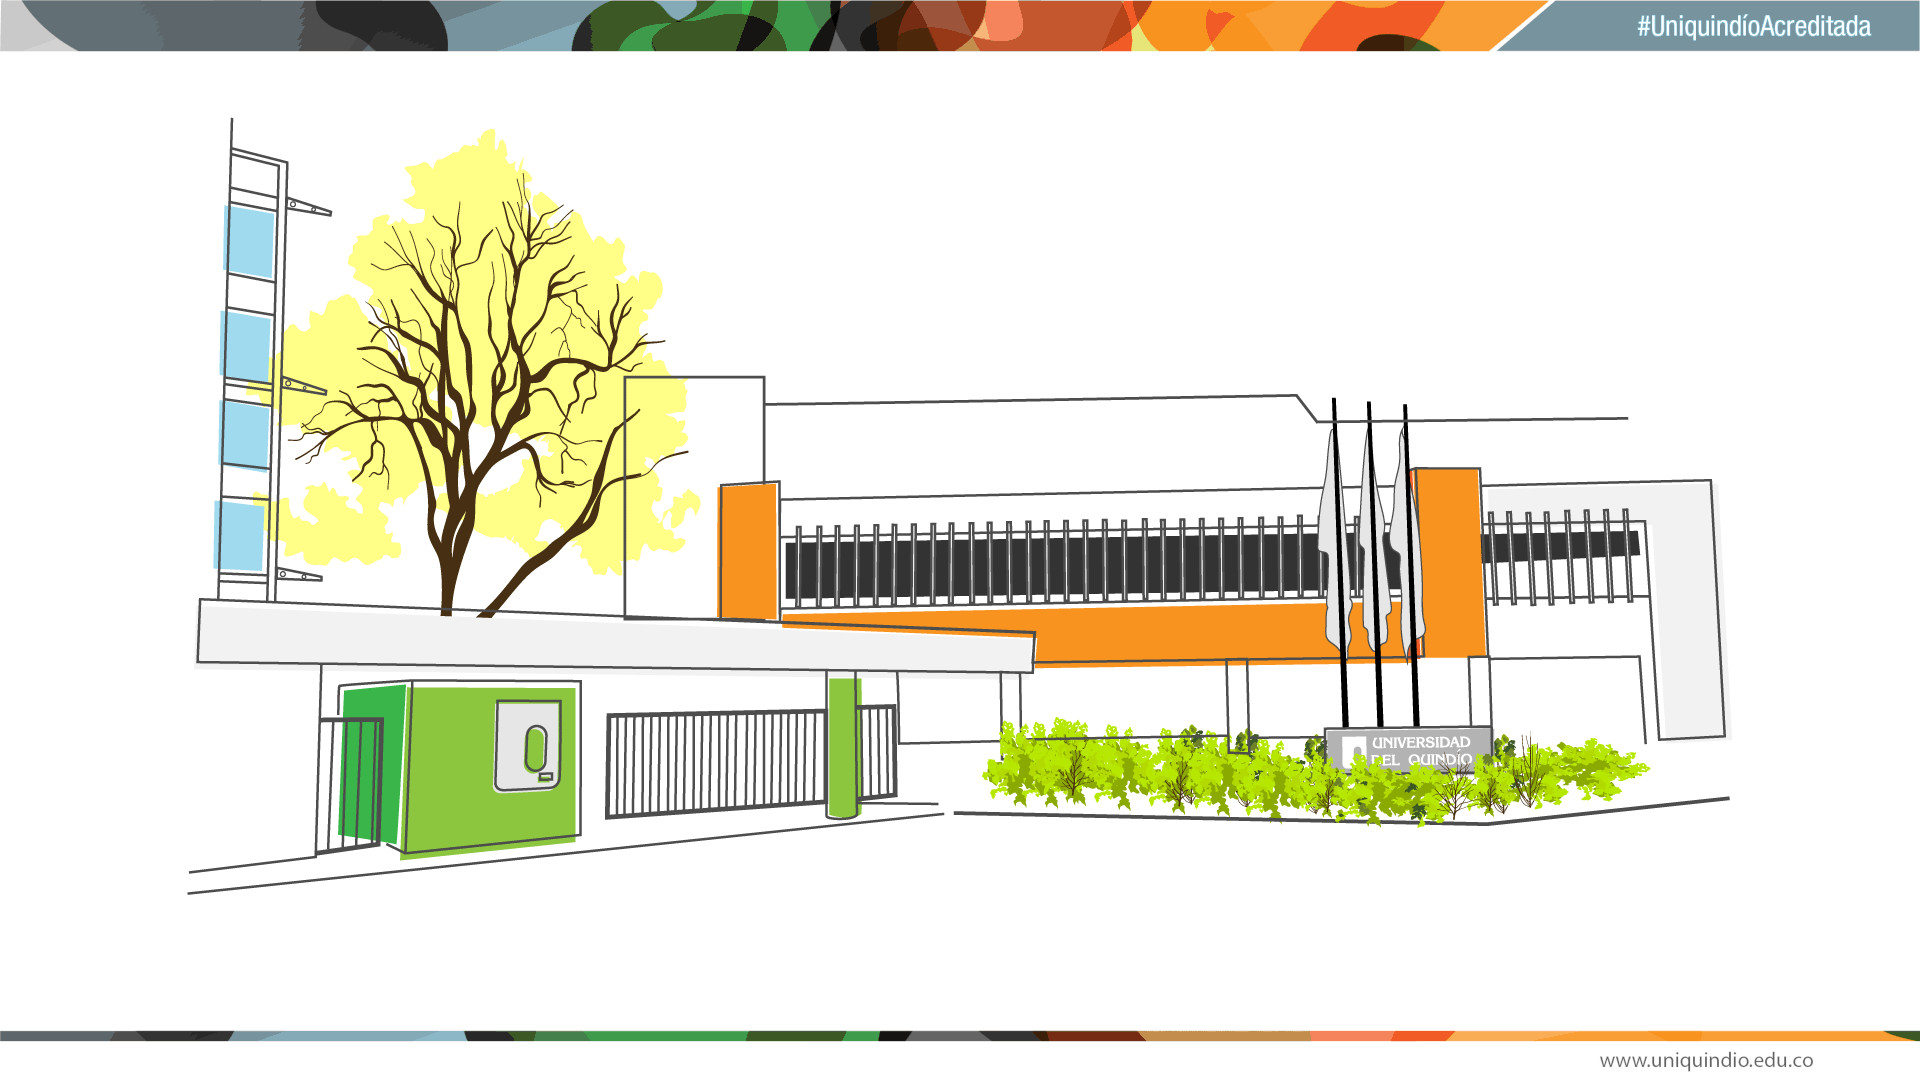
\includegraphics[width=\paperwidth,height=\paperheight]{Imagenes/portada.jpg}}

\begin{document}
	
	\frame{\titlepage}
	
	\setbeamertemplate{background canvas}{
\includegraphics[width=\paperwidth,height=\paperheight]{Imagenes/fondo2.jpg}}
	
	\begin{frame}
		\frametitle{Contenido}
			\tableofcontents[hideallsubsections]
	\end{frame}

%\begin{frame}
%	\begin{block}{Titulo}
%		Contenido
%	\end{block}
%\end{frame}

	 	\section{Introducción}
\frametitle{Introducción}

 A lo largo del crecimiento de los entornos inteligentes, como Smart House, se han realizado investigaciones con múltiples orientaciones, las cuales están enfocadas en razones sociales como la comodidad y la seguridad, sin dejar de lado factores ambientales como el ahorro energético. En cuanto a una parte más técnica, estos procesos inteligentes se componen por software, hardware y firmware.\\
 
 Las investigaciones hacia el ámbito de Smart House se enfocan en monitorear y/o controlar múltiples aspectos de una casa. Para realizar esta tarea físicamente se usa un hardware, en el cual se ven inmersos la unidad central de procesamiento, los sensores y los actuadores; la primera se encarga del monitoreo y control del entorno.\\
 
 Autores como Behan \cite{Behan2013} y Cheuque \cite{Cheuque2015} han usado mini computadoras o computadoras de placa simple (SBC), como lo es Raspberry Pi, siendo esta una unidad central o unidad de mando, permitiendo el control de la iluminación en la casa. Sin embargo, no solo se usan tarjetas de prototipado, también se construyen nuevos dispositivos con funciones más específicas, así como Kusriyanto \cite{Kusriyanto2015}, el cual usó un microcontrolador ATmega 16, contando con más pines, representa otro modo de hacer eficiente el uso del hardware.\\
 
 En Smart House, se ha implementado variedad de software, usado para la conexión entre los dispositivos móviles y el central, más aun, que sea posible controlar la casa o realizar la comunicación entre el dispositivo central y los esclavos. Del mismo modo, con el fin de ejecutar diferentes tareas como enviar datos al servidor, entre otras.\\
 
 Así, por ejemplo, Cheuque \cite{Cheuque2015} ha desarrollado una aplicación basada en PHP, usando servidores Web como Lighttpd, el cual se soporta en PostgreSQL para las bases de datos; esta aplicación se conecta a la unidad central de procesamiento con el fin de monitorear y controlar cargas LED; teniendo esto en cuenta, realizar aplicaciones en PHP es muy usado a fin de controlar la casa, sea localmente o desde la web como realizo Kasmi \cite{Kasmi2016}. Otro servidor externo, Heroku, el cual fue usado por Kaneko \cite{Kaneko2017} para la visualización de datos desde cualquier lugar, sin necesidad de tener el servidor local compartido a internet.\\
 
 Los dispositivos inteligentes aumentan a gran velocidad, por la necesidad de estar siempre conectados, dando paso a aplicar esta conexión a diferentes espacios del hogar; una casa inteligente o Smart House se compone de multiples artefactos que se encuentran enlazados a la red con posibilidad de acceso desde cualquier parte del mundo. \\
 
 En este trabajo se realiza la construcción completa de una solución para Smart House, desarrollando el hardware, firmware y software. El hardware cuenta con múltiples entradas con el fin de monitorear el entorno de aplicación por medio de sensores, también posee salidas enfocadas a cargas AC y DC, en busca de gestionar y controlar dicho ámbiente. El software se ve reflejado en el desarrollo de una aplicación web, cuya característica principal es el panel de control, donde se muestran los valores de los sensores y asimismo los estados de las cargas junto con su correspondiente control de forma simple para el usuario, de tal manera que a través del firmware e internet se vinculen las interacciones generadas y recibidas en el software con su respectiva carga o sensor en el hardware. Además de esto, se desarrolla una prueba Beta, la cual cuenta con diferentes ítems enfocados en evaluar la interacción del usuario con la totalidad del sistema, de tal manera que sea posible determinar su desempeño.\\
 
 Este trabajo está organizado en siete capítulos. El lector en el capítulo 2 encontrará la descripción del objetivo general y objetivos específicos. En el capítulo 3 se encuentra recopilado el marco teórico, distribuido en conceptos importantes de IoT, así como también del Hardware y el Software en cuestión. El capítulo 4 presenta el desarrollo, pasando por la construcción del hardware y la creación del firmware y software. Los resultados se encuentran plasmados en el capítulo 5. En el capítulo 6 se muestran las conclusiones y en el capítulo 7 están los trabajos futuros, por último el glosario, la bibliografía y los Anexos.\\
 

 
 	\begin{frame}
		\section{Objetivos}
\frametitle{Objetivos}

\subsection{Objetivo General}

Desarrollar una solución IoT para una habitación en un entorno de Smart House.

\subsection{Objetivos Específicos}

- Desarrollar un prototipo de una tarjeta inalámbrica para una habitación en un entorno Smart House.

- Desarrollar una aplicación web encargada de permitir la interacción del usuario con su habitación.

- Evaluar el desempeño del sistema en una prueba beta.
 	\end{frame}
 	
 	\frametitle{Marco Teórico}
\section{Internet de las Cosas}

La internet de las cosas es un sistema de dispositivos de computación interrelacionados, máquinas mecánicas y digitales, objetos, animales o personas que tienen identificadores únicos y la capacidad de transferir datos a través de una red, sin requerir de interacciones humano a humano o humano a computadora. \\

IoT ha evolucionado desde la convergencia de tecnologías inalámbricas, sistemas micro-electromecánicos, microservicios e Internet. La convergencia ha ayudado a derribar las paredes de silos entre la tecnología operativa y la tecnología de la información, permitiendo que los datos no estructurados generados por máquinas sean analizados para obtener información que impulse mejoras. \cite{TechT2017}\\

Kevin Ashton, cofundador y director ejecutivo del Auto-ID Center de MIT, mencionó por primera vez la internet de las cosas en una presentación que hizo a Procter \& Gamble en 1999. He aquí cómo Ashton explica el potencial del internet de las cosas:

``Las computadoras de hoy –y, por lo tanto, la internet– dependen casi totalmente de los seres humanos para obtener información. Casi todos los aproximadamente 50 petabytes (un petabyte son 1.024 terabytes) de datos disponibles en internet fueron capturados y creados por seres humanos escribiendo, presionando un botón de grabación, tomando una imagen digital o escaneando un código de barras. \\

El problema es que la gente tiene tiempo, atención y precisión limitados, lo que significa que no son muy buenos para capturar datos sobre cosas en el mundo real. Si tuviéramos computadoras que supieran todo lo que hay que saber acerca de las cosas –utilizando datos que recopilaron sin ninguna ayuda de nosotros– podríamos rastrear y contar todo, y reducir en gran medida los desechos, las pérdidas y el costo. Sabríamos cuándo necesitamos reemplazar, reparar o recordar cosas, y si eran frescas o ya pasadas”. \cite{Asthon2009}

\subsection{Plataforma Heroku}

``Heroku es una plataforma en la nube basada en un sistema gestionado por contenedores, con servicios de datos integrados y un potente ecosistema para desarrollar y ejecutar aplicaciones modernas. La experiencia de los desarrolladores de Heroku es un enfoque centrado en aplicaciones para la entrega de software, integrado con las herramientas y flujos de trabajo de desarrollador más populares de la actualidad'' \cite{Hero}.


\subsection{Framework Laravel}

``Laravel es un framework de aplicaciones web con una sintaxis expresiva y elegante. Laravel intenta aliviar el dolor del desarrollo al facilitar las tareas comunes que se utilizan en la mayoría de los proyectos web, como la autenticación, el enrutamiento, las sesiones y el almacenamiento en caché.\\

Laravel tiene como objetivo hacer que el proceso de desarrollo sea agradable para el desarrollador sin sacrificar la funcionalidad de la aplicación. Con este fin, se ha intentado combinar lo mejor de lo que hemos visto en otros marcos web, incluidos los marcos implementados en otros lenguajes, como Ruby on Rails, ASP.NET MVC y Sinatra.\\

Laravel es accesible, pero potente, y proporciona potentes herramientas necesarias para aplicaciones grandes y robustas. Una magnífica inversión de contenedores de control, un sistema de migración expresivo y un soporte de prueba de unidades estrechamente integrado le brindan las herramientas que necesita para construir cualquier aplicación'' \cite{Lara}.

\subsection{HTTP}

El protocolo de transferencia de hipertexto (HTTP) es un protocolo de la capa de aplicación en el modelo OSI, usado para transmitir documentos hipermedia como HTML. Diseñado con el propósito de la comunicación entre navegadores y servidores web, no obstante, puede operar con otros propósitos. HTTP sigue un modelo clásico de cliente-servidor, con un cliente que abre una conexión y realiza una petición a la espera de respuesta. HTTP es un protocolo sin estado, significa que el servidor no conserva ningún dato entre dos solicitudes. Para realizar las peticiones, este protocolo cuenta con diferentes metodos \cite{HTTP}.

Metodos de solicitud HTTP:

HTTP define un conjunto de métodos de solicitudes para indicar la acción deseada que se realizará a un recurso determinado. Aunque pueden ser sustantivos, estos métodos algunas veces se denominan verbos HTTP. Cada uno de ellos implementa una semántica diferente, pero algunas características comunes son compartidas por un grupo de ellos \cite{HTTPM}.\\

\begin{itemize}
	\item GET: este método solicita una representación del recurso especificado. Las peticiones que lo usan, solo deben regresar datos.
	\item HEAD: este método solicita una respuesta igual a una peticion GET, pero sin el cuerpo de la respuesta.
	\item POST: se usa para enviar una entidad al recurso especificado, causando a menudo un cambio en el estado o efectos secundarios en el servidor.
	\item PUT: reemplaza todas las representaciones actuales del recurso destino con la la petición de carga útil.
	\item DELETE: esta petición elimina el recurso especificado.
	\item CONNECT: establece un túnel para el servidor identificado por el recurso de destino.
	\item OPTIONS: se usa para describir las opciones de la comunicación para el recurso destino.
	\item TRACE: realiza una prueba de mensaje loop-back a lo largo de la ruta del recurso de destino. 
	\item PATCH: se usa para realizar modificaciones parciales a un recurso.
\end{itemize}

\subsection{JSON}

``JSON (JavaScript Object Notation - Notación de Objetos de JavaScript) es un formato ligero de intercambio de datos. Leerlo y escribirlo es cómodo para los humanos, al igual que para las máquinas resulta simple interpretarlo y generarlo. Está basado en un subconjunto del Lenguaje de Programación JavaScript, Standard ECMA-262 3rd Edition - Diciembre 1999. JSON es un formato de texto que es completamente independiente del lenguaje pero utiliza convenciones que son ampliamente conocidos por los programadores de la familia de lenguajes C, incluyendo C, C++, C\#, Java, JavaScript, Perl, Python, y muchos otros. Estas propiedades hacen que JSON sea un lenguaje ideal para el intercambio de datos'' \cite{JSON}.\\

JSON está constituído por dos estructuras:

\begin{itemize}
	\item Una colección de pares de nombre/valor. En varios lenguajes esto es conocido como un objeto, registro, estructura, diccionario, tabla hash, lista de claves o un arreglo asociativo.
	
	\item Una lista ordenada de valores. En la mayoría de los lenguajes, esto se implementa como arreglos, vectores, listas o secuencias.
\end{itemize}

Estas son estructuras universales; virtualmente todos los lenguajes de programación las soportan de una forma u otra. Es razonable que un formato de intercambio de datos que es independiente del lenguaje de programación se base en estas estructuras \cite{JSON}.

\subsection{Base de Datos}

``Se define una base de datos como una serie de datos organizados y relacionados entre sí, los cuales son recolectados y explotados por los sistemas de información de una empresa o negocio en particular.

Cada base de datos se compone de una o más tablas que guarda un conjunto de datos. Cada tabla tiene una o más columnas y filas. Las columnas guardan una parte de la información sobre cada elemento que queramos guardar en la tabla, cada fila de la tabla conforma un registro'' \cite{DB}. \\

Para la gestión de datos es muy común encontrar las funciones básicas de crear, leer, actualizar y borrar (CRUD), con la finalidad de que el usuario final pueda acceder a estos sin necesidad de realizar peticiones directamente a la base de datos, sino en una interfaz gráfica (GUI).

\section{Smart House}

El concepto de Smart House implica tres características básicas. En primer lugar, el monitoreo a través de redes de sensores para obtener información sobre la casa y sus residentes. En segundo lugar, los mecanismos que controlan el uso de la comunicación entre dispositivos con el fin de permitir la automatización y el acceso remoto. Por último, las interfaces de usuario, como los teléfonos inteligentes y las computadoras que permiten a los usuarios especificar las preferencias, así como presentar información a las personas acerca de estas. \\

Smart House es un entorno que tiene sistemas sofisticados a través de los cuales se pueden controlar algunos de los objetos de la casa, como luces, puertas, ventanas, además puede racionalizar el consumo de energía, entre otras funciones mediante el uso de sensores. Básicamente, uno de los beneficios más importantes del uso de la tecnología en las casas, es la prestación de servicios a las personas.\cite{Howedi2016} 

\section{Hardware}

\subsection{ESP-WROOM-32}

Es un potente módulo MCU Wi-Fi + BT + BLE que se dirige a una amplia variedad de aplicaciones, desde redes de sensores de baja potencia hasta las tareas más exigentes, como codificación de voz, transmisión de música y decodificación de MP3, además de su reducido tamaño, según se observa en la figura \ref{fig:esp32-wroom-s32-00}.\\

En el núcleo de este módulo está el chip ESP32-D0WDQ6. El chip integrado se encuentra diseñado para ser escalable y adaptable. Hay dos núcleos de CPU que se pueden controlar individualmente, y la frecuencia del reloj es ajustable de 80 MHz a 240 MHz. El usuario también puede apagar la CPU y utilizar el coprocesador de baja potencia para monitorear constantemente los periféricos en busca de cambios o cruces de umbrales. ESP32 integra un amplio conjunto de periféricos, que van desde sensores táctiles capacitivos, sensores Hall, interfaz de tarjeta SD, Ethernet, SPI de alta velocidad, UART, I2S e I2C.\\

La integración de Bluetooth, Bluetooth LE y Wi-Fi garantiza que se pueda orientar una amplia gama de aplicaciones, el uso de Wi-Fi permite un gran alcance físico y conexión directa a Internet a través de este, mientras usa Bluetooth, le permite al usuario conectarse convenientemente al teléfono o transmitir balizas de baja energía para su detección. La corriente de reposo del chip ESP32 es inferior a 5 uA, lo que lo hace adecuado para aplicaciones de electrónica con batería y portátiles. ESP32 admite una velocidad de datos de hasta 150 Mbps y una potencia de salida de 20.5 dBm en la antena con el objetivo de garantizar el rango físico más amplio.\\

El sistema operativo elegido para ESP32 es freeRTOS con LwIP; TLS 1.2 con aceleración de hardware está integrado también, además se admite la actualización segura (cifrada) a través del aire (OTA), de modo que los desarrolladores puedan actualizar continuamente sus productos incluso después de su lanzamiento.\cite{EW32}

%\begin{figure}[H]
%	\centering
%	\caption{ESP WROOM 32. Tomado de: \cite{ESPIMG}}
%	\label{fig:esp32-wroom-s32-00}
%	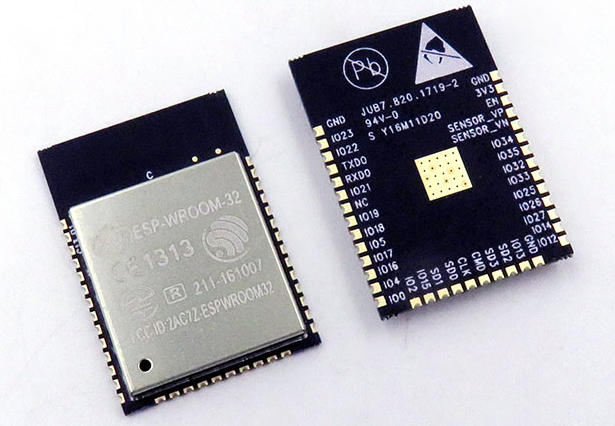
\includegraphics{Imagenes/esp32-wroom-s32-00}
%\end{figure}

\subsection{Corriente Alterna (AC)}

``Es un tipo de corriente eléctrica, en la que la dirección del flujo de electrones va y viene a intervalos regulares o en ciclos. La corriente que fluye por las líneas eléctricas y la electricidad disponible normalmente en las casas procedente de los enchufes de la pared es corriente alterna. La corriente estándar utilizada en los EE.UU. es de 60 ciclos por segundo (es decir, una frecuencia de 60 Hz); en Europa y en la mayor parte del mundo es de 50 ciclos por segundo (es decir, una frecuencia de 50 Hz.)''. \cite{Cor}

\subsection{Corriente Directa (DC)}

``Es la corriente eléctrica que fluye de forma constante en una dirección, como la que fluye en una linterna o en cualquier otro aparato con baterías es corriente continua.

Una de las ventajas de la corriente alterna es su relativamente económico cambio de voltaje. Además, la pérdida inevitable de energía al transportar la corriente a largas distancias es mucho menor que con la corriente continua''. \cite{Cor}

\subsection{Control de potencia AC por ángulo de fase}

``Los SCR y los TRIAC, permiten aplicar una técnica muy conveniente y eficaz para controlar el voltaje promedio y por lo tanto la potencia aplicada a una carga, cambiando el ángulo de fase con el cual la fuente de voltaje se aplica a ésta. Esta técnica de control de voltaje es muy usada en las aplicaciones de regulación de motores, iluminación y temperatura, por ser el voltaje la variable principal en estos tres procesos''.\cite{CEKIT}\\

``Para entender como se controla el ángulo de fase, por medio de un TRIAC conectado en serie con la carga, se puede asumir que el TRIAC se comporta idealmente como un interruptor controlador por la corriente de compuerta Ig que se cierra o se abre ante su presencia o ausencia. Observando la figura \ref{fig:triacgraph} puede verse el control de una onda seno de tensión con un período con un período de 360 grados; en la parte (a) de la figura se muestra la tensión a través del TRIAC, mientras que en la parte (b) se ve la tensión sobre la carga; allí puede verse que el TRIAC se comporta como un circuito abierto durante los primero 45 grados de cada semiciclo, y todo el voltaje cae en sus terminales eliminando el flujo de corriente por la carga. La porción del semiciclo durante la cual se presenta esta situación se conoce como ángulo de disparo''\cite{CEKIT}.\\

``Una vez el TRIAC es disparado a través de su terminal de compuerta (G), éste se engancha y se comporta como un interruptor cerrado, permitiendo que todo el voltaje se aplique a la carga durante los 135 grados restantes de cada semiciclo. La porción del semiciclo durante la cual el TRIAC conduce se denomina ángulo de conducción''\cite{CEKIT}.

%\begin{figure}[H]
%	\centering
%	\caption{Representación gráfica del ángulo de disparo y de conducción del TRIAC y de la carga. Tomado de: \cite{CEKIT}.}
%	\label{fig:triacgraph}
%	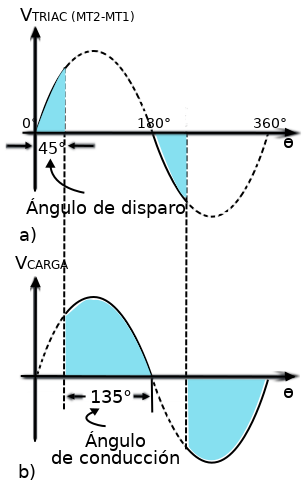
\includegraphics[width=0.3\linewidth]{Imagenes/TRIAC_graph}
%\end{figure}

\subsection{Control de Cargas DC}

Los transistores como switch permiten controlar las cargas de corriente continua con ayuda de una señal PWM que los activa o desactiva. Las cargas de corriente continuas típicas como los motores y LED's, a parte de poder funcionar en dos estados, encendido y apagado, pueden se controladas mediante la modulación por ancho de pulso (PWM), ya que al variar el ancho de pulso de la señal eléctrica se varia la cantidad de energía entregada a la carga, por ejemplo, si es un LED el cambio se refleja en su intensidad lumínica y si es un motor DC cambia su velocidad de giro \cite{PWM}. Este control se produce gracias a que en esta modulación se modifica su ciclo útil, cambiando el tiempo en que la señal eléctrica se encuentra en alto durante un periodo, por lo tanto si el ciclo útil es del 10\% el poder entregado es poco, en comparación, con un ciclo útil del 50\% o 100\% conforme se observa en la figura \ref{fig:pwm-duty-800x396}.

%\begin{figure}[H]
%	\centering
%	\caption{Ciclo Útil PWM. [Imagen Propia] }
%	\label{fig:pwm-duty-800x396}
%	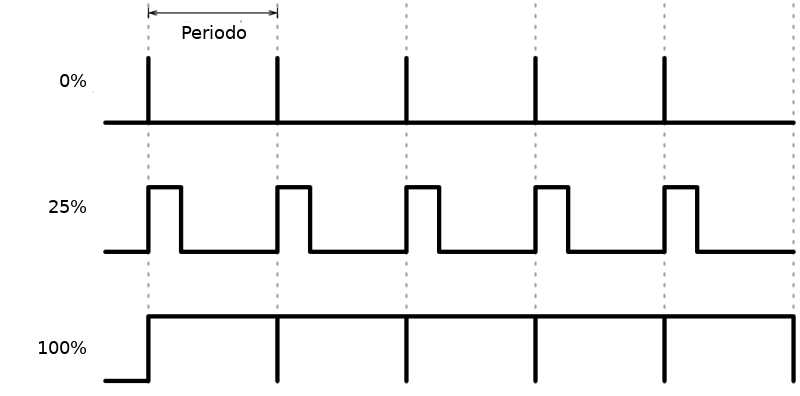
\includegraphics[width=0.5\linewidth]{Imagenes/pwm}
%\end{figure}


\subsection{I2C}

``I2C es un puerto y protocolo de comunicación serial, define la trama de datos y las conexiones físicas para transferir bits entre 2 dispositivos digitales. El puerto incluye dos cables de comunicación, SDA y SCL. Además el protocolo permite conectar hasta 127 dispositivos esclavos con esas dos líneas, con hasta velocidades de 100, 400 y 1000 kbits/s. También es conocido como IIC ó TWI – Two Wire Interface'' \cite{I2C}.

\subsection{Sensores}

\subsubsection{Módulo GY-30}

``Sensor GY-30 BH1750FVI. Es un sensor digital de intensidad de luz ambiente, tiene un conversor ADC de 16bits interno y comunicación por I2C como se observa en la figura \ref{fig:gy-30}. Esta es una versión mejorada del típico sensor de luz a base de un LDR, el cual simplemente entrega un valor analógico. Compatible con Arduino, PIC, etc. \\

El módulo BH1750 es un sensor de luz, que a diferencia del LDR es digital y nos entrega valores de medición en Lux ( lumen /m$^2$ ) que es una  unidad de medida estándar para el nivel de iluminación (iluminancia). Tiene alta precisión y un rango ente 1 – 65535 lx el cual es configurable.\\

La interfaz de comunicación es I2C pudiéndolo implementar en la mayoría de micro controladores, el módulo aparte de los pines de alimentación y pines I2C tiene un pin para establecer la dirección''.\cite{GY30}

%\begin{figure}[H]
%	\centering
%	\caption{Modulo GY-30. Tomado de: \cite{GY30}}
%	\label{fig:gy-30}
%	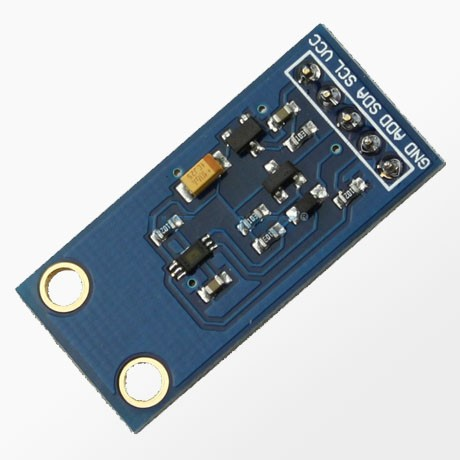
\includegraphics[width=0.4\linewidth]{Imagenes/gy-30}
%\end{figure}

\subsubsection{Temperatura y Humedad DHT11}

``El DHT11 es un sensor de temperatura y humedad digital de bajo costo. Utiliza un sensor capacitivo de humedad y un termistor para medir el aire circundante, y muestra los datos mediante una señal digital en el pin de datos (no hay pines de entrada analógica). Es bastante simple de usar, pero requiere sincronización cuidadosa para tomar datos. El único inconveniente de este sensor es que sólo se puede obtener nuevos datos una vez cada 2 segundos, así que las lecturas que se pueden realizar serán mínimo cada 2 segundos''. \cite{DHT11}

%\begin{figure}[H]
%	\centering
%	\caption{Sensor de temperatura y humedad DHT11. Tomado de: \cite{DHT11}}
%	\label{fig:dht11}
%	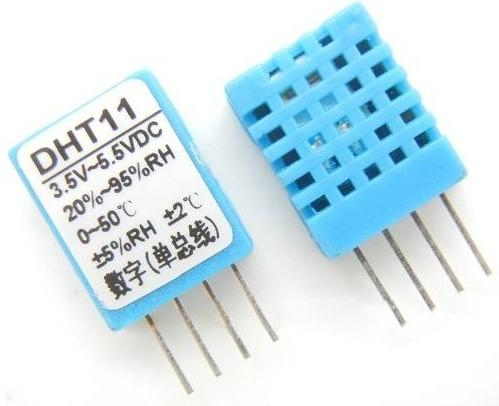
\includegraphics[width=0.4\linewidth]{Imagenes/dht11}
%\end{figure}


\subsubsection{Módulo sensor de calidad de aire MQ-135}

La serie MQ de sensores de gas son sensores analógicos, por lo cual son fáciles de implementar con cualquier microcontrolador que posea un conversor analógico digital (ADC) adecuado. Estos detectores son electroquímicos y cambian su resistencia con la exposición a determinados gases, internamente poseen un calentador que se encarga de aumentar la temperatura interna para que el sensor pueda reaccionar con los gases provocando un cambio de valor en la resistencia, su estructura interior se puede observar en la figura \ref{fig:estructura-del-sensor-mq}.\cite{MQ1}

%\begin{figure}[H]
%	\centering
%	\caption{Estructura del sensor MQ. Tomado de: \cite{MQ1}}
%	\label{fig:estructura-del-sensor-mq}
%	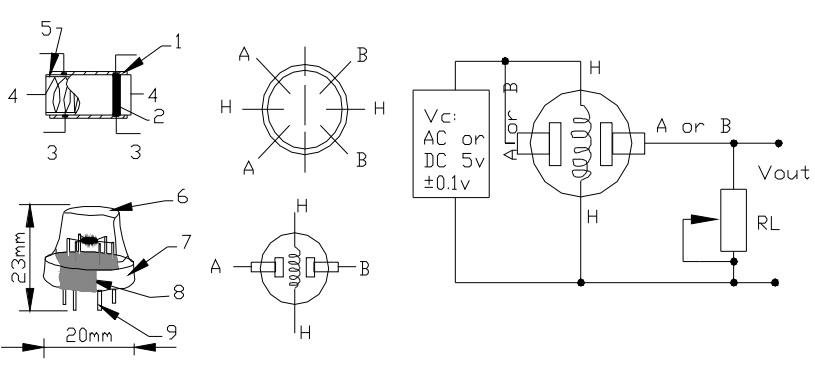
\includegraphics[width=0.7\linewidth]{Imagenes/Estructura_del_sensor_MQ}
%\end{figure}

El Sensor Calidad Aire MQ135 se utilizan en equipos de control de calidad del aire a edificios y oficinas, son adecuados para la detección de NH3, NOx, alcohol, benceno, humo, CO2, etc; además de que estos sensores vienen en módulos como se observa en la figura \ref{fig:sensor-calidad-aire-mq135}, lo que facilita su uso, simplemente se debe conectar al microcontrolador sin necesidad de utilizar algún circuito de acople. \cite{MQ1}

%\begin{figure}[H]
%	\centering
%	\caption{Modulo sendor de calidad de Aire MQ-135. Tomado de: \cite{MQ1}}
%	\label{fig:sensor-calidad-aire-mq135}
% 	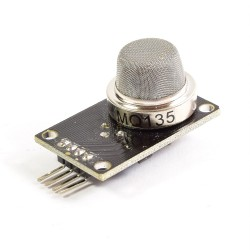
\includegraphics[width=0.35\linewidth]{Imagenes/sensor-calidad-aire-mq135}
%\end{figure}

Este sensor es sensible en similar proporción a los gases mencionados, con lo que se puede determinar si el aire está limpio o si existe presencia de algún gas nocivo.\\

Los datos de salida de este sensor no son valores absolutos, simplemente proporciona una salida analógica que se debe monitorear y ser comparada con los valores típicos proporcionados en la hoja de datos.\cite{MQ2}

\subsubsection{Sensores de Estado}

Los sensores de estado describen si la variable esta en alto (1) o en bajo (0), para estos detectores se tienen variables típicas, como el estado de una puerta o una ventana (abierta o cerrada), la lluvia, el movimiento.

Módulo detector de lluvia: 

Es un módulo relativamente simple que consiste en una serie de pistas conductoras organizadas de forma paralela e impresas sobre una placa de baquelita como se observa en la figura \ref{fig:yl-83}. La separación entre sus caminos es muy pequeña, con el fin de crear un corto circuito cada vez que las pistas se mojan, ya que es un circuito abierto y el agua hace que se cree un camino de baja resistencia entre las pistas que tienen diferente potencial (Vcc-GND). La corriente que fluye a través de estas pistas se ve limitada por resistencias de 10K en cada conductor, lo que impide que el corto circuito que se genera cuando se moja la placa vaya a estropear el micro controlador.\cite{LLU}

%\begin{figure}[H]
%	\centering
%	\caption{Sensor de Lluvia. Tomado de: \cite{LLU}}
%	\label{fig:yl-83}
%	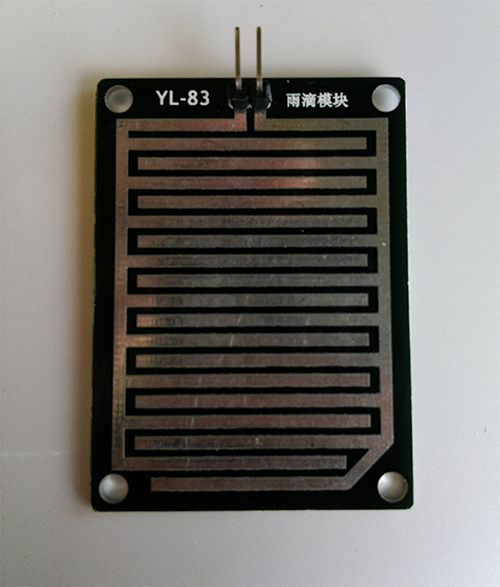
\includegraphics[width=0.35\linewidth]{Imagenes/YL-83}
%\end{figure}

El circuito de control es el que posee las resistencias limitadoras de corriente y es el encargado de alimentar el módulo de la figura \ref{fig:yl-83}. Como se observa en la figura \ref{fig:yl-831} tiene un amplificador operacional, específicamente el circuito integrado LM392. Este se ocupa de amplificar el pequeño diferencial de voltaje que se produce cuando una gota de agua cae sobre las pistas del módulo. Aquí es donde se genera la señal de salida que puede ser del tipo analógica o digital. La señal digital oscilará entre los valores HIGH y LOW dependiendo de si hay agua o no sobre las pistas de la placa.\\

La salida analógica entregará un nivel de voltaje que variará dependiendo de la cantidad de agua que haya sobre el módulo.\cite{LLU}\\

%\begin{figure}[H]
%	\centering
%	\caption{Modulo de sensor de lluviar. [Imagen Propia]}
%	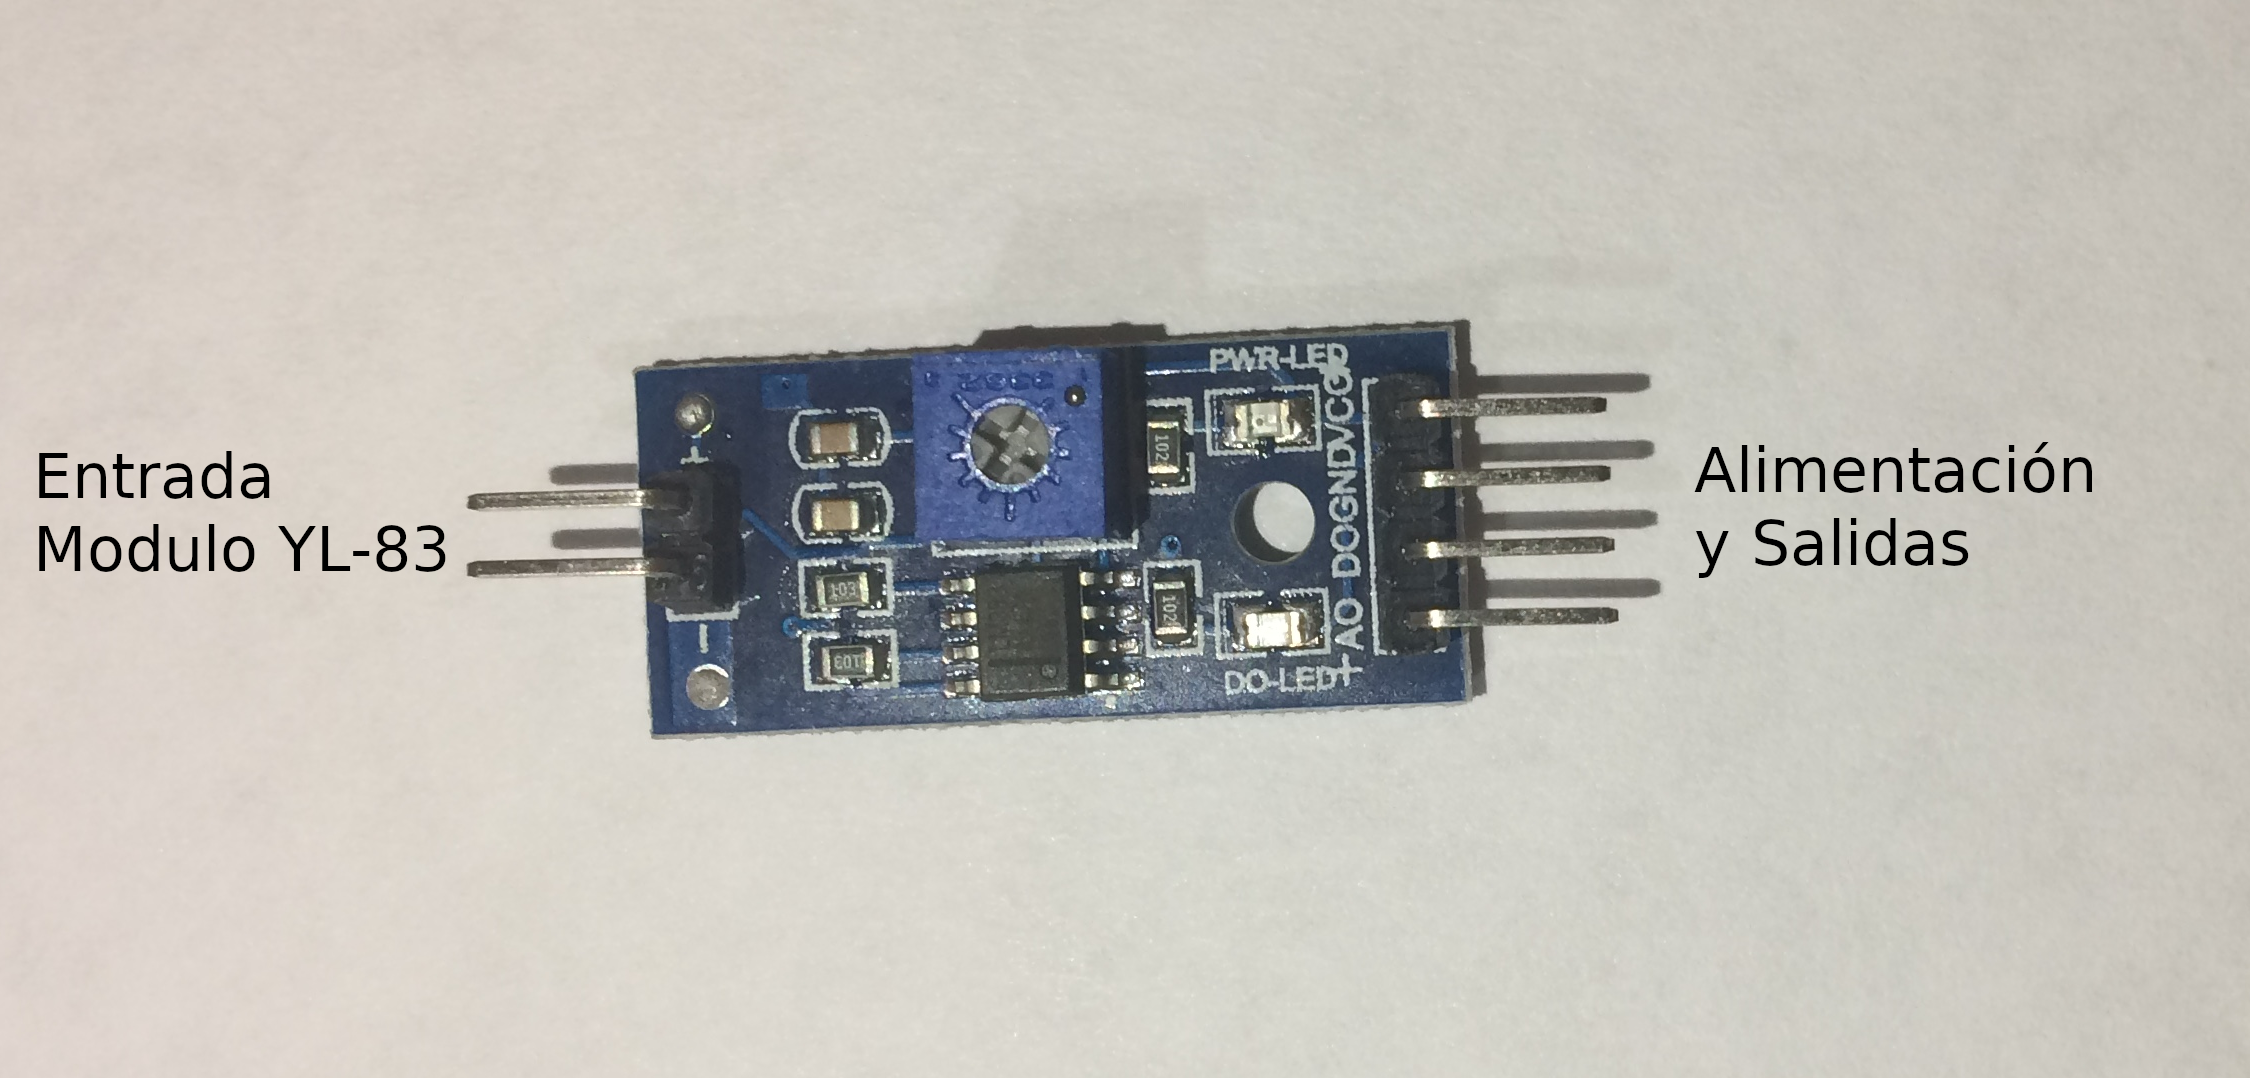
\includegraphics[width=0.5\linewidth]{Imagenes/YL-831}
%	\label{fig:yl-831}
%\end{figure}

Módulo PIR HC-SR501: 

La función de los sensores PIR es detectar movimiento, normalmente se busca detectar el movimiento de una persona dentro del rango del sensor. Son baratos, pequeños, de bajo consumo y fáciles de utilizar, además no se desgastan. Habitualmente se encuentran en electrodomésticos y gadgets para la oficina o el hogar. Son conocidos como PIR, ``Sensores Infrarrojos'' o ``Sensores de movimiento''.\\

Este módulo contiene un sensor Piroelectrico, el cual puede detectar niveles de radiación infrarroja como se observa en la figura \ref{fig:sensor-hc-sr501-1000-m}. El detector de movimiento está dividido en dos mitades, la razón para esto es que se busca la diferencia en el movimiento y no el promedio. Las dos mitades están unidas de modo que se cancelan una a otra. Entonces, si una mitad recibe más o menos radiación IR, la salida cambiará a Alto o Bajo. \cite{PIR1}\\

El módulo PIR modelo HC-SR501, es pequeño y de bajo costo como se observa en la figura \ref{fig:sensor-hc-sr501-1000-m}, incorpotando la tecnología más reciente en sensores infrarrojos pasivos para detectar movimiento. La emisión infrarroja se da en personas por su temperatura corporal y en animales (mamíferos), ya que emiten una radiación similar a los humanos. \cite{PIR2}

%\begin{figure}[H]
%	\centering
%	\caption{Sensor HCSR501. Tomado de: \cite{PIR2}}
%	\label{fig:sensor-hc-sr501-1000-m}
%	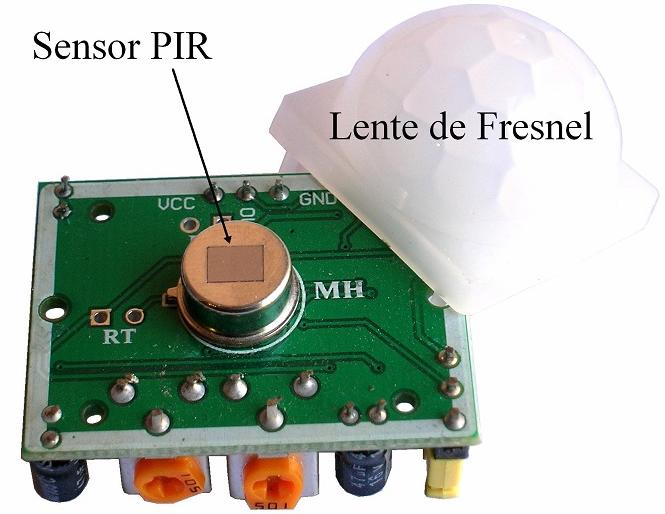
\includegraphics[width=0.5\linewidth]{Imagenes/SENSOR-HC-SR501-1000-M}
%\end{figure}

\section{Software}

\subsection{RTOS}

Los sistemas operativos en tiempo real, tienen como parámetro clave al tiempo, ya que en gran variedad de situaciones, por ejemplo, un proceso industrial, se requiere recolectar múltiples datos, los cuales son usados para el control de diversos procesos que deben ser ejecutados en determinados instantes, de no ser así, podría causar desde la mala ejecución de una tarea, hasta un accidente según la delicadeza del proceso.\\ 

Para procesos con nula tolerancia a fallos, se conoce como un sistema en tiempo real duro, muchos de estos sistemas se encuentran en el control de procesos industriales, en aeronáutica, en la milicia y en áreas de aplicación similares. el caso contrario, cuando se tiene cierta permisividad a que muy ocasionalmente existan errores, se conoce como sistema en tiempo real suave, los sistemas de audio digital o de multimedia están en esta categoría. Los teléfonos digitales también son ejemplos de sistema en tiempo real suave. \cite{SO} \\

``Como en los sistemas en tiempo real es crucial cumplir con tiempos predeterminados para realizar una acción, algunas veces el sistema operativo es simplemente una biblioteca enlazada con los programas de aplicación, en donde todo está acoplado en forma estrecha y no hay protección entre cada una de las partes del sistema. Un ejemplo de este tipo de sistema en tiempo real es freeRTOS.  Las categorías de sistemas para computadoras de bolsillo, sistemas integrados y sistemas en tiempo real se traslapan en forma considerable. Casi todos ellos tienen por lo menos ciertos aspectos de tiempo real suave. Los sistemas integrados y de tiempo real sólo ejecutan software que colocan los diseñadores del sistema; los usuarios no pueden agregar su propio software, lo cual facilita la protección. \\

Los sistemas de computadoras de bolsillo y los sistemas integrados están diseñados para los consumidores, mientras que los sistemas en tiempo real son más adecuados para el uso industrial. Sin embargo, tienen ciertas características en común''. \cite{SO}

\subsection{ESP-IDF}

ESP-IDF es el entorno de desarrollo oficial para el ESP32 desarrollado por Espressif System, el cual mediante una serie de comandos específicos escritos en la terminal (en el caso de linux), habilita la configuración del ESP32 en cuanto a su funcionamiento, es decir, permite encender o apagar características como el WiFi, el Bluetooth o realizar particiones de memoria, ademas de esto, se puede cargar el código por el puerto USB al ESP32, al igual que visualizar la información generada por el ESP32 por el mismo puerto. Este entorno se encuentra construido con diferentes características y APIs, algunas de ellas se mencionan a continuación. \cite{ES}

\subsection{Proteus}

Proteus combina facilidad de uso con características de gran alcance con la finalidad de ayudar a diseñar, probar y concebir PCB profesionales. Con casi 800 variantes de microcontroladores listos para la simulación directamente desde el esquematico, además de contar con uno de los paquetes de diseño de PCB profesionales más intuitivas en el mercado y un autoruteo de clase mundial incluido como estándar. \cite{Prot1} \\

Además es una herramienta muy completa y potente de simulación de circuitos y diseño de PCBs. Dentro de la simulación de circuitos admite componentes pasivos, digitales, analógicos y componentes más complejos como LCDs y motores. Por tanto, se puede realizar casi cualquier cosa, el programa está pensado para que una vez se tenga el circuito diseñado se pueda pasar a una PCB \cite{Prot2}. Adicionalmente los dispositivos que no se encuentren se pueden agregar, ya sea de la pagina oficial o construyendolos en el software por medio de las funcionalidades provistas.

 	
 	\section{Desarrollo}

\subsection{Hardware}\label{sec:hw}

El prototipo para Smart House tiene por objetivo monitorear el entorno de aplicación y controlarlo por medio de mecanismos como motores o dispositivos de iluminación, razón por la cual está equipada con etapas de potencia de corriente alterna y directa, etapa de adquisición de datos, entre otras características que permitan cumplir con los objetivos planteados.\\ 

El prototipo fue diseñado en el software Proteus, desde el esquemático hasta la placa de circuito impreso (PCB), en la figura \ref{fig:esp32} se observa el esquematico de la tarjeta ESP32 construido junto con su distribución de pines, además de sus conexiones correspondientes dentro de este programa. El prototipo está separado en dos secciones, la etapa de potencia AC y la etapa DC, en la última, se encuentra la mayor parte de circuitos que funcionan con corriente directa.\\

\begin{figure}[H]
	\centering
	\caption{ESP32 creado en proteus [Imagen Propia]}
	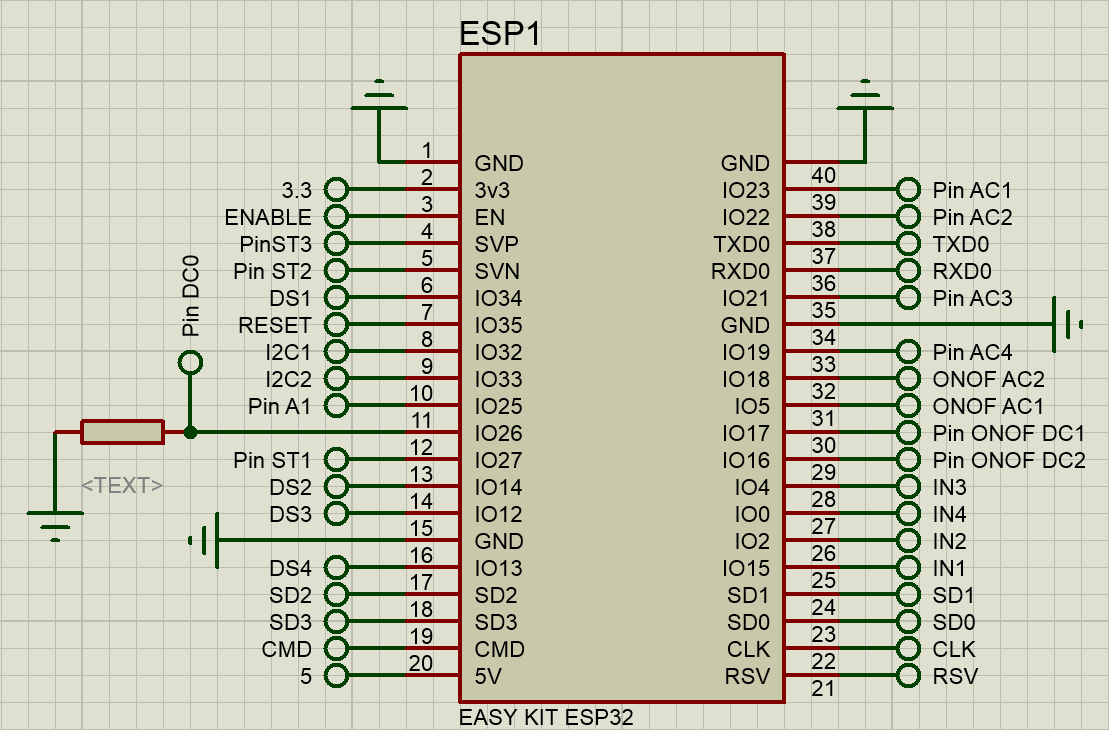
\includegraphics[width=0.5\linewidth]{Imagenes/ESP32}	
	\label{fig:esp32}
\end{figure}

En los siguientes ítems se resaltaran las características más importantes que lleva el circuito:\\

	\subsection{Alimentacion}
	
	Corriente alterna (AC):
		El prototipo recibe el voltaje directamente de la red eléctrica a la que se encuentra conectado el entorno de aplicación, el cual está pensado para una habitación dentro de una Smart House; en el caso de Colombia, la red doméstica comúnmente otorga 110V AC, los cuales son regulados para el funcionamiento adecuado del prototipo, como la etapa de potencia AC y el detector de cruce por cero con el fin de sincronizar la tarjeta a dicha red eléctrica.\\
		
	Corriente directa (DC):
		Para la alimentación DC del circuito, se hace uso de un conversor AC-DC que regula el voltaje de la red eléctrica a 12V DC, con los cuales se manejara la etapa de potencia DC, además de ser usados por dos modulos conversores DC-DC, mostrados en la figura \ref{fig:DCDC}, ambos con entradas de 12V DC y con salidas a los niveles lógicos comunes, 5V y 3.3V, empleados con el fin de alimentar dispositivos como optoacopladores, transistores BJT o relevadores con activación de 5V, así como también la tarjeta de prototipo ESP32.\\
		
		Cabe resaltar que la tarjeta permite una entrada externa de 12VDC a 5A si se desean controlar cargas a un máximo de 50W.\\
			
		\begin{figure}[H]
			\centering
			\caption{Modulo conversor DC-DC. Tomado de: \cite{DCDC}}
			\label{fig:DCDC}
			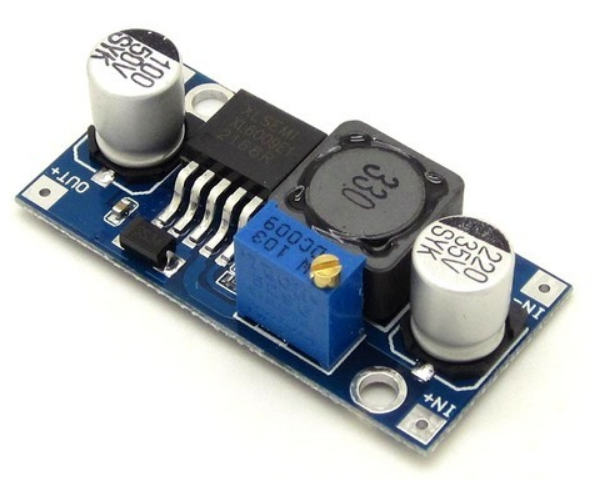
\includegraphics[width=0.5\linewidth]{Imagenes/DCDC}
		\end{figure}
	
	\subsection{Entradas}
	Sensores:
		El prototipo viene equipado con una etapa de adquisición de datos con capacidad entre 7 a 134 sensores, pues posee una entrada I2C, ampliando el número de dispositivos conectados, lo cual también permitiría adicionar tareas más específicas en escenarios que lo requieran.\\
		
		Con la finalidad de realizar pruebas del prototipo, se hacen uso de 5 sensores para medir magnitudes y situaciones en el entorno, tal como calidad del aire, temperatura, humedad, luz visible, movimiento y presencia de lluvia, debido a que estas medidas o estados se encuentran en casi cualquier ambiente. Teniendo en cuenta que el ESP32 funciona en voltajes lógicos de 3.3V, se tienen 4 entradas de sensores directamente conectados a los pines de la tarjeta, con la capacidad de cambiar el voltaje de alimentación para 3 de ellos, como se muestra en la figura \ref{fig:SVS}, pues en el mercado se encuentran sensores que manejan voltajes de alimentación ya sea de 3.3V o 5V, mientras que la cuarta entrada se encuentra alimentada con 5V, ya que tiene un uso específico en las pruebas para el sensor de calidad de aire, esta viene acondicionada con un diodo zener en contraposición, para evitar que la tarjeta ESP32 tenga un voltaje de entrada superior a 3.3V, según se observa en la figura \ref{fig:S1Aire}.\\
		
		Las tres entradas para sensores de estado (ST1, ST2, ST3), a diferencia de las demás, se encuentran conectadas a pines de la tarjeta que no presentan resistencia de pull down por software, por ello se agregan estas al sistema, tal como se observa en la figura \ref{fig:ST}.\\
		
		\begin{figure}[H]
			\centering
			\caption{Entrada de sensores[Imagen Propia]}
			\label{fig:SVS}
			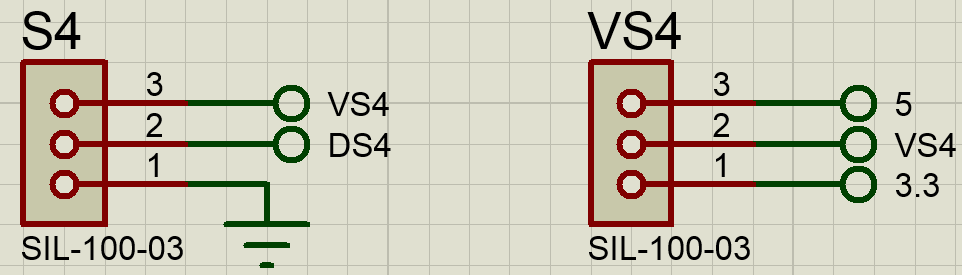
\includegraphics[width=0.7\linewidth]{Imagenes/SVS}
		\end{figure}
	
		\begin{figure}[H]
			\centering
			\caption{Entrada para sensor de calidad de aire[Imagen Propia]}
			\label{fig:S1Aire}
			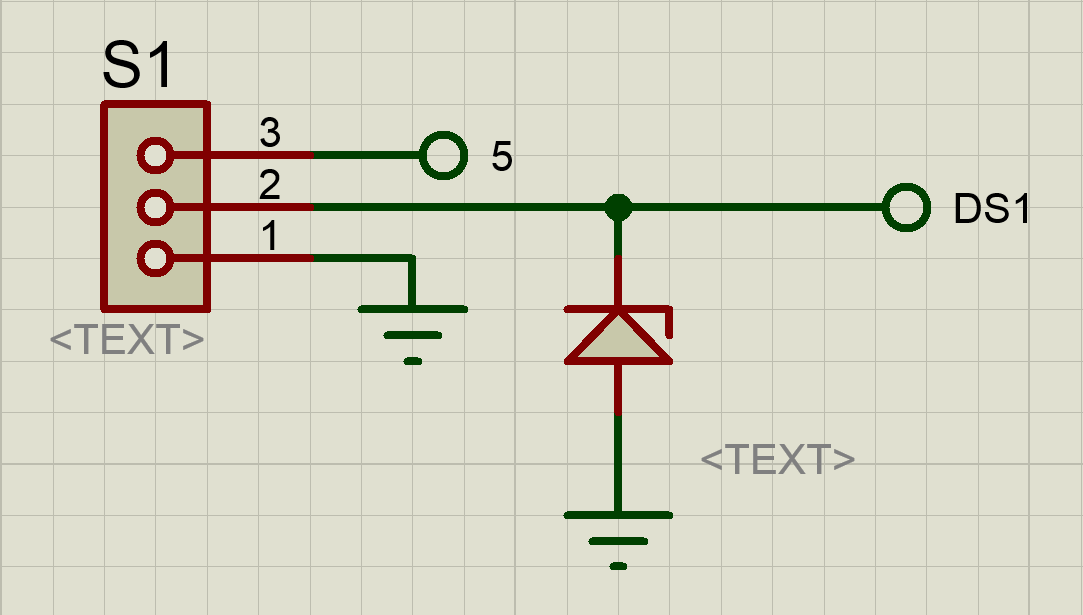
\includegraphics[width=0.6\linewidth]{Imagenes/S1Aire}
		\end{figure}
	
		\begin{figure}[H]
			\centering
			\caption{Entrada para sensores con resistencia de pull down[Imagen Propia]}
			\label{fig:ST}
			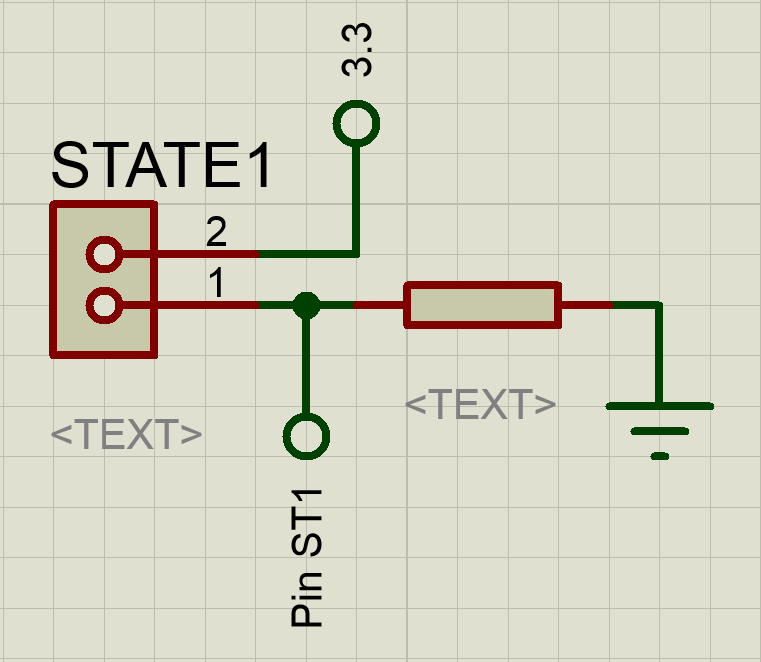
\includegraphics[width=0.5\linewidth]{Imagenes/ST}
		\end{figure}		
	
	Calibración de audio:
		Para calibrar la salida audible se hace uso de una resistencia variable (Potenciometro), el cual permite regular el voltaje de entrada al circuito de amplificación mostrado en la figura \ref{fig:AUD}; este será descrito en el presente capitulo en la sección de salidas del hardware.\\ 
		
	Botón enable:
		Presionando el botón enable se reinicia la tarjeta ESP32, junto con su firmware.\\
		
	Botón reset:
		Presionando el botón reset se borran las credenciales ingresadas para la conexión del ESP32 a la red wifi.\\
		
	\subsection{Salidas:}
	Etapa de potencia AC:
		Se encuentra diseñada a una potencia de 2000W en un total de seis cargas, cuatro de ellas cuentan con un circuito para el control por ángulo de fase, como se observa en la figura \ref{fig:CAC1}, con una capacidad individual de 500W, gracias a el TRIAC BTA26600, mostrado en la figura \ref{fig:TRIAC}, el cual soporta una corriente máxima de 25A. Con el fin de proteger el ESP32, se hace uso de optoacopladores MOC3021, debido a su funcionalidad para aislar circuitos de forma óptica.\\
		
		\begin{figure}[H]
			\centering
			\caption{Control por angulo de fase [Imagen Propia]}
			\label{fig:CAC1}
			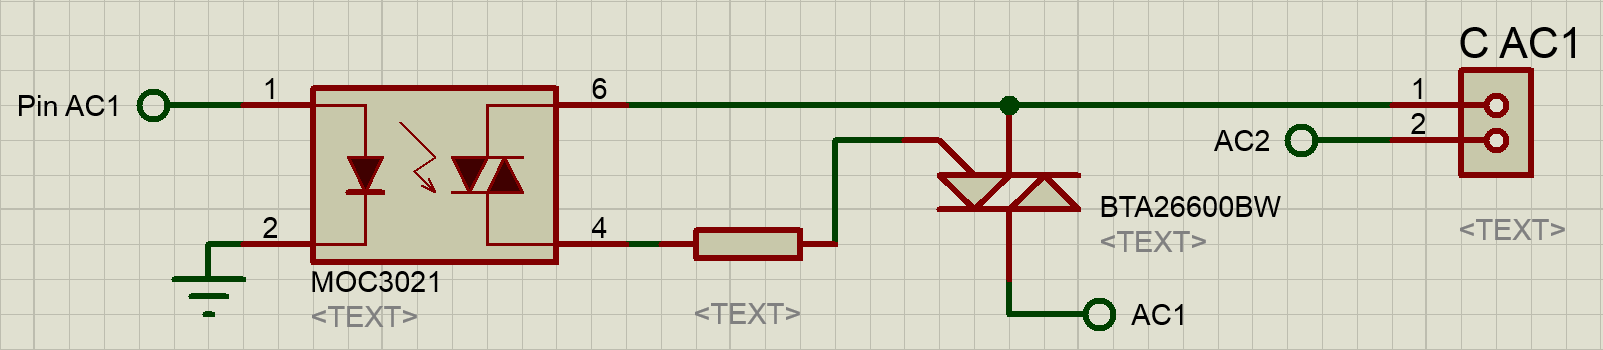
\includegraphics[width=0.8\linewidth]{Imagenes/CAC1}
		\end{figure}
	
		\begin{figure}[H]
			\centering
			\caption{Triac BTA26600. Tomado de: \cite{TRIAC}}
			\label{fig:TRIAC}
			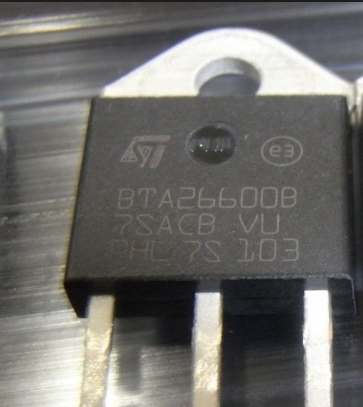
\includegraphics[width=0.35\linewidth]{Imagenes/TRIAC}
		\end{figure}
	
		Las dos cargas restantes corresponden a un sistema de encendido y apagado, cuyo funcionamiento se basa en un relevador SRA-05VDC-CL activado a 5V por medio de un transistor BJT como switch, gracias a este relé, las salidas tienen capacidad de hasta 200W cada una, en la figura \ref{fig:ONOFAC} se observa el circuito diseñado en proteus. Para proteger el ESP32 el prototipo se vale de ese dispositivo, puesto que presenta un aislamiento magnético por la naturaleza de su operación.\\
	
		\begin{figure}[H]
			\centering
			\caption{Interruptor para cargas AC [Imagen Propia]}
			\label{fig:ONOFAC}
			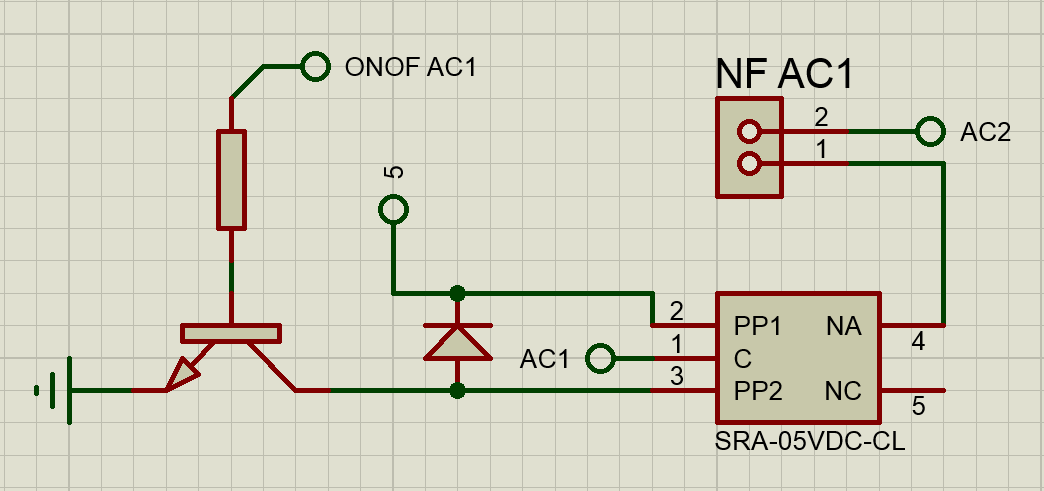
\includegraphics[width=0.7\linewidth]{Imagenes/ONOFAC}
		\end{figure}
	
		Dentro de la etapa AC se encuentra el detector de cruce por cero, el cual cuenta con un fototransistor 4N25, debido a su alta capacidad de aislamiento, tomando la onda rectificada completa y pasándola a un nivel lógico de 3.3V, esta parte del circuito se observa en la figura \ref{fig:DC01}; para que la señal sea más confiable se hace uso de un Schmitt-Trigger CD40106 mostrado en la figura \ref{fig:DC02}, valiéndose de la histéresis de voltaje garantizando que la señal de salida sea poco susceptible al ruido \cite{DC0}.\\
		
		\begin{figure}[]
			\centering
			\caption{Detector de cruce por cero [Imagen Propia]}
			\label{fig:DC01}
			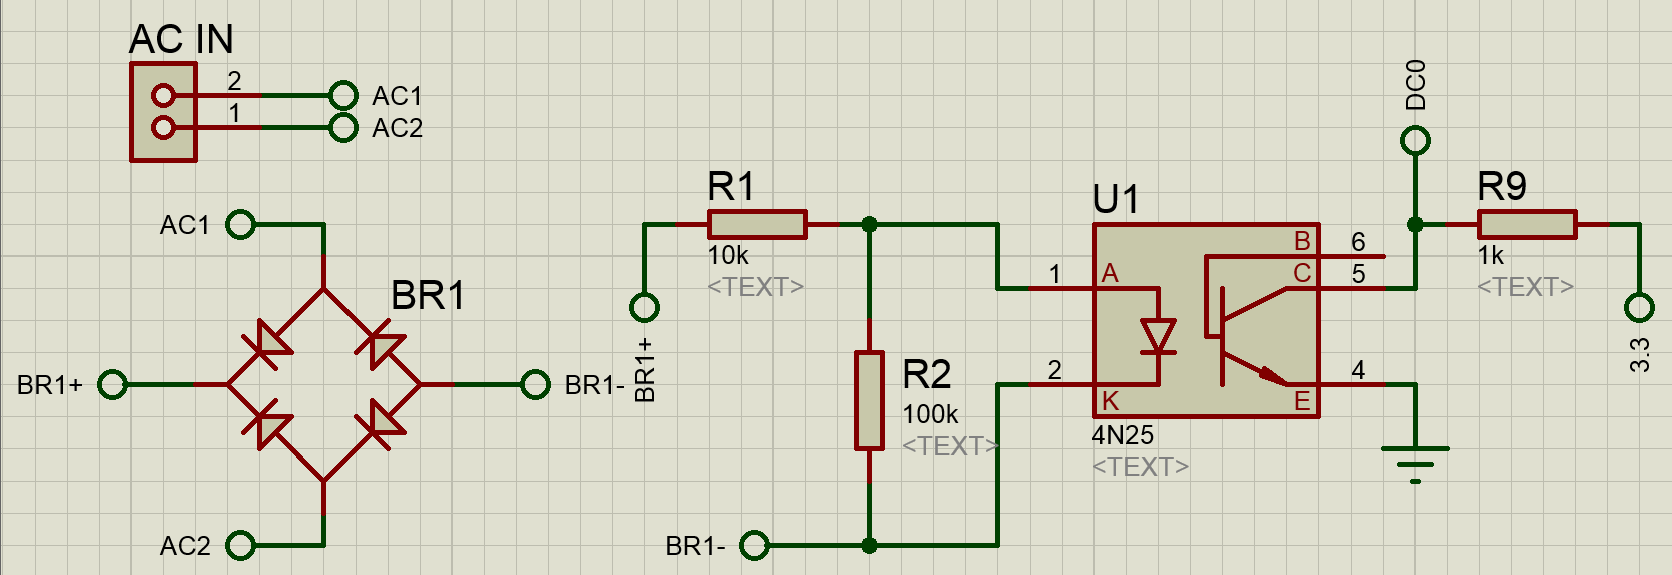
\includegraphics[width=0.85\linewidth]{Imagenes/DC01}
		\end{figure}
	
		\begin{figure}[]
			\centering
			\caption{Schmitt trigger para el detector de cruce por cero [Imagen Propia]}
			\label{fig:DC02}
			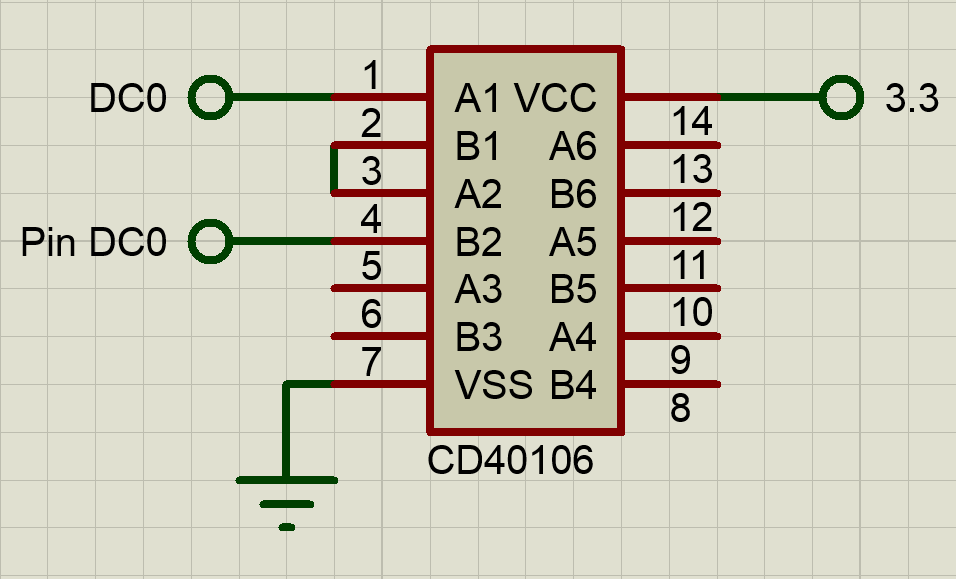
\includegraphics[width=0.5\linewidth]{Imagenes/DC02}
		\end{figure}
	
	Etapa DC:
		Esta etapa cuenta con cuatro salidas de control diseñadas para cargas de 12V, de las cuales, dos de ellas tienen un enfoque a motores, puesto que está equipada con control de velocidad a base de PWM e inversión de giro con un puente h usando transistores mosfet IRLZ44N; el puente h se encuentra controlado por un circuito integrado L293D, que garantiza un voltaje Vgs adecuado para la correcta activación del los transistores; este circuito se muestra en la figura \ref{fig:L293D} y \ref{fig:CDC}.\cite{IRL}.\\
		
		Las dos salidas restantes también cuentan con mosfet IRLZ44N, y su control igualmente es a base de PWM, mas no permite realizar la inversión de giro, por lo cual se enfoca a dispositivos como lámparas LEDs, el diseño en proteus se muestra en la figura \ref{fig:ONOFDC}.\\
		
		\begin{figure}[H]
			\centering
			\caption{Integrado L293D [Imagen Propia]}
			\label{fig:L293D}
			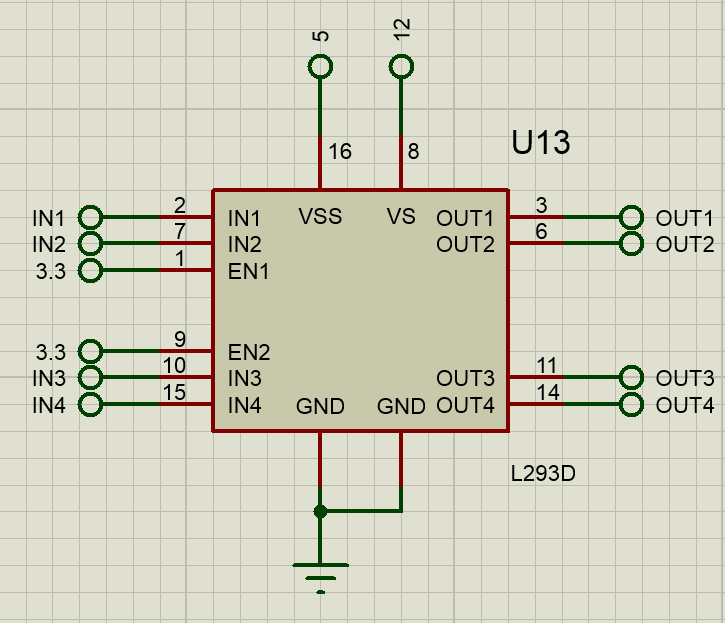
\includegraphics[width=0.5\linewidth]{Imagenes/L293D}
		\end{figure}
		
		\begin{figure}[H]
			\centering
			\caption{Puente h para control de motores DC [Imagen Propia]}
			\label{fig:CDC}
			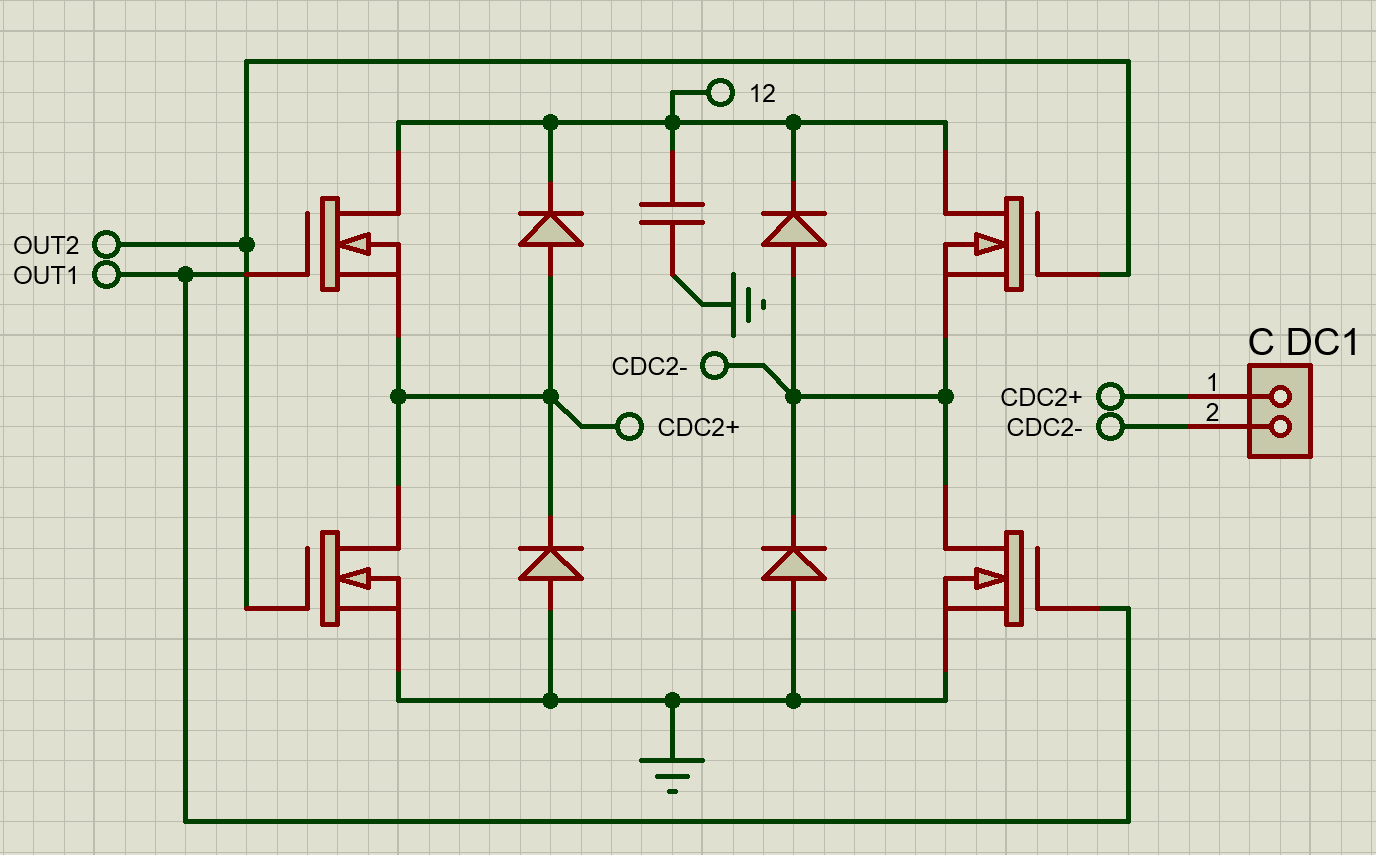
\includegraphics[width=0.7\linewidth]{Imagenes/CDC}
		\end{figure}
	
		\begin{figure}[H]
			\centering
			\caption{Control para cargas DC [Imagen Propia]}
			\label{fig:ONOFDC}
			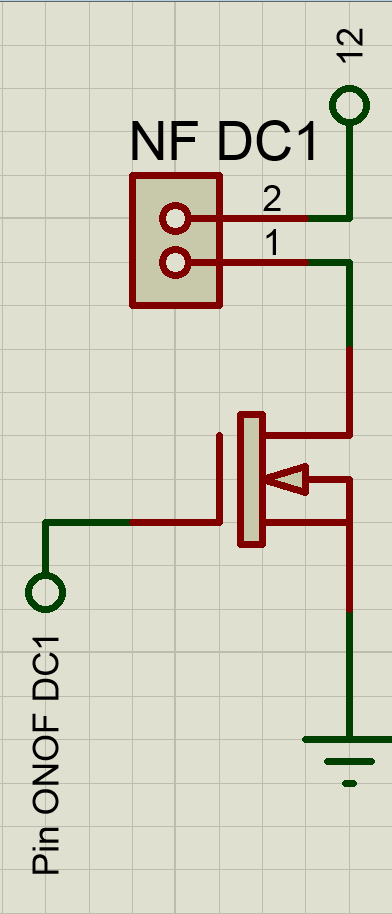
\includegraphics[width=0.25\linewidth]{Imagenes/ONOFDC}
		\end{figure}
	
	Salida audible:
		Está diseñada para emitir sonidos a una sola frecuencia, o sonido mono estéreo, caso dado cuando se activa una regla programada en la aplicación web, enfocada a las cargas de encendido y apagado, tanto de la etapa de potencia AC como la etapa DC; el sonido emitido por el prototipo corresponde a una voz con tonalidad femenina, pronunciando el estado en el cual se configura la carga según la regla (ya sea encendido, o apagado).\\
		
		El circuito utilizado para la salida audible está basado en el amplificador de audio LM386, implementando el esquema típico de aplicación ilustrado en su datasheet \cite{LM386}, en la figura \ref{fig:AUD} se observa implementado en el software proteus.\\
		
		Como se mencionó anteriormente, el circuito presenta un potenciómetro a la entrada para calibrar el voltaje de esta, con el obejtivo de no saturarla y que la salida sea lo mas fiel posible.\\
		
		\begin{figure}[H]
			\centering
			\caption{Circuito tipico para el LM386 [Imagen Propia]}
			\label{fig:AUD}
			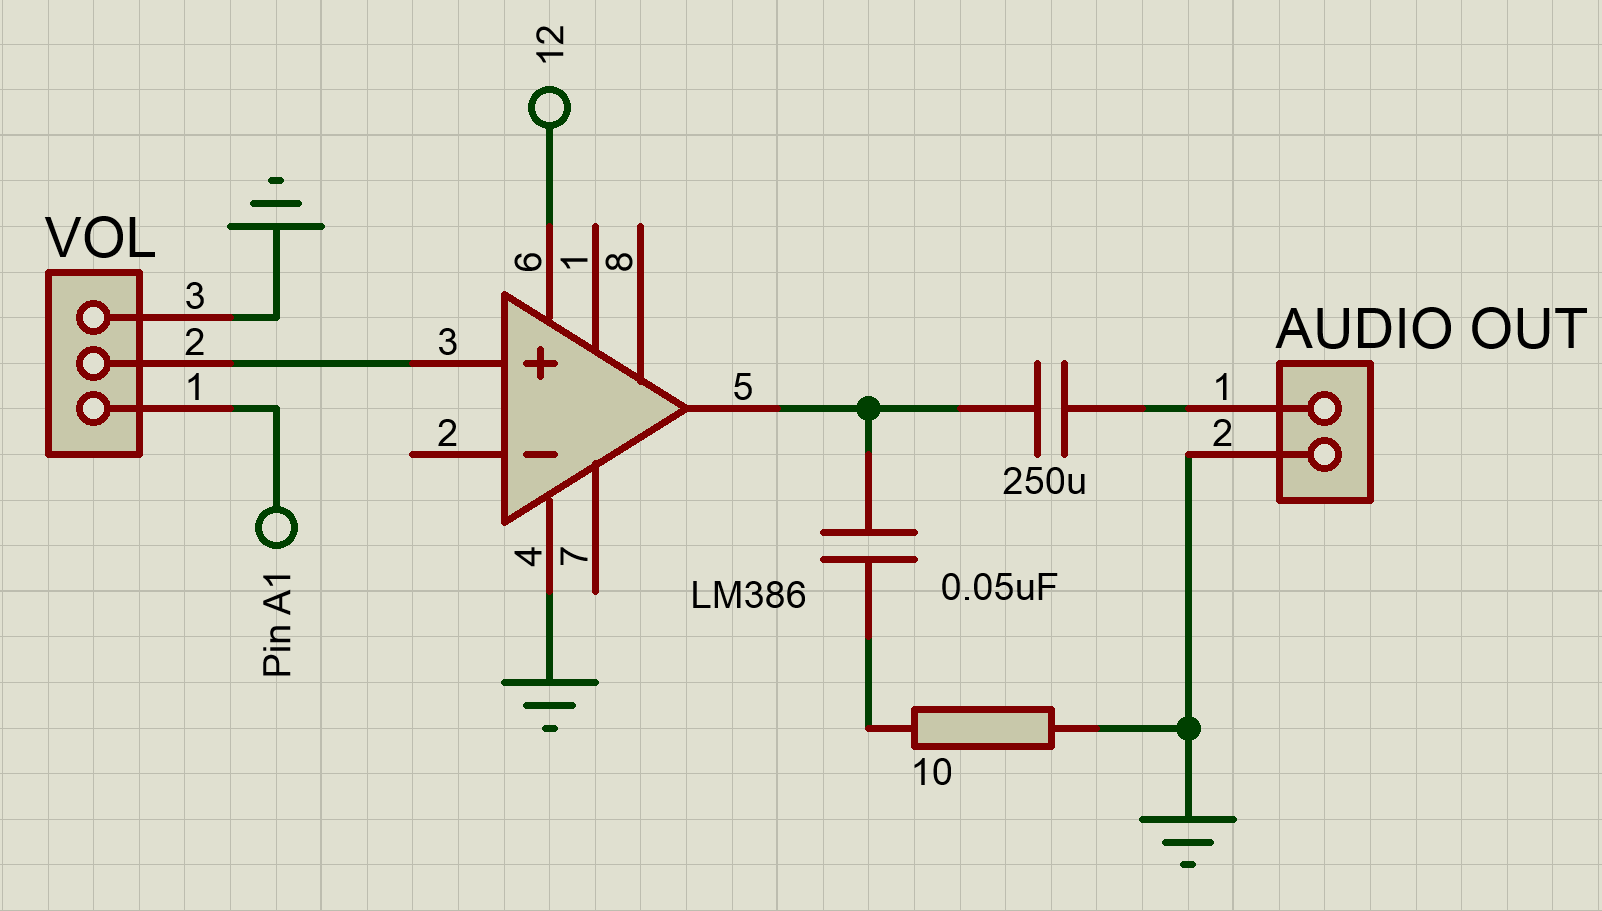
\includegraphics[width=0.7\linewidth]{Imagenes/AUD}
		\end{figure}		
				
\section{Firmware}

El firmware se desarrolla sobre el framework o SDK oficial de Espressif Systems ESP-IDF, el cual posee una documentación \cite{ES} muy útil a la hora de utilizar las diferentes APIs presentes en este; para el desarrollo de la aplicación es necesario contar con los requisitos que se observan en la figura \ref{fig:what-you-need}. Esta característica del sistema incluye un kernel de tiempo real llamado FreeRTOS, el cual da soporte al manejo de los diversos recursos del sistema; al ser un RTOS, las funciones se definen mediante tareas, entonces cada funcionalidad de la tarjeta o grupo de funcionalidades se desarrolla en una o varias tareas que realicen las acciones adecuadas, por ejemplo, en el caso de los sensores, cada uno tiene una tarea para la lectura y gestión de datos, así como también ocurre de manera similar con las salidas de la tarjeta, pues cuentan con tareas encargadas de la gestión del encendido y apagado, asimismo para el control de cargas, ya sea por ángulo de fase o PWM.\\

\begin{figure}[H]
	\centering
	\caption{ESP-IDF. Tomado de: \cite{ES}}
	\label{fig:what-you-need}
	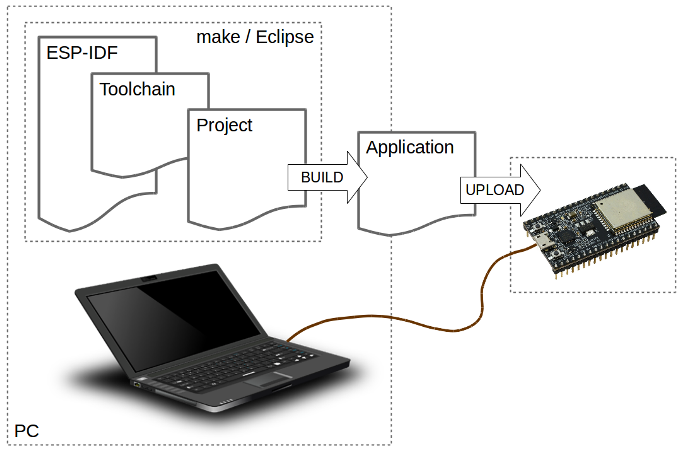
\includegraphics[width=0.5\linewidth]{Imagenes/what-you-need}
\end{figure}


Sobre el firmware se desarrollan los siguientes temas:

Tareas:

Se ejecutan constantemente en el sistema operativo, realizando diferentes funciones para lectura, escritura y control.

GPIO:

El ESP-WROOM-32 posee diferentes GPIO, los cuales se usan para leer o escribir señales digitales; en cuanto a los sensores, se pueden enviar señales con el fin de iniciar su lectura o simplemente tener el pin en modo entrada y leerlo cada cierto intervalo de tiempo generando datos de lectura, o en modo salida para el control de los diversos dispositivos que se han desarrollado en el hardware.

ADC,DAC:

Los ADC se usan para leer los datos de algunos sensores que proporcionan señales analógicos, por este motivo se hace la conversión de la señal analógica a un valor digital dentro de la tarjeta, así luego identificar el dato de la lectura del sensor. Los DAC son usados para realizar la operación contraria, es decir, teniendo valores digitales convertirlos a un valor analógico por ejemplo generar audios o diferentes señales a partir del software.

%\paragraph{Consola:}para realizar diferentes pruebas directamente desde la tarjeta, se usa la opción de la consola, la cual se comunica por medio del puerto serie, para esto se crean las funciones y los comandos que estaran disponibles; algunos son \textit{http}, para ejecutar las peticiones http manualmente y observar su respuesta, \textit{pin} para realizar la prueba de un pin digital como entrada o salida, \textit{help} para observar la lista de comandos, entre otros.

HTTP Request:

Las peticiones HTTP son indispensables en estas aplicaciones del campo IOT, por tal motivo en el desarrollo del firmware se usan las librerias pertinentes para realizarlas y además leer las respuestas de estas desde el servidor, ya que este es el medio de comunicación tarjeta-servidor.

Hora de Red:

Se obtiene la hora mediante el protocolo simple de tiempo de red (SNTP), este resulta de gran utilidad para la sincronización de los relojes de los sistemas informáticos. Se mantiene actualizada con el objetivo de realizar diferentes acciones respecto a esta.

Timers:

La tarjeta posee dos grupos de timers y cada uno tiene dos timers, un timer lo usa el sistema operativo, otro es configurado con el fin de realizar el control de potencia AC por ángulo de fase, para tener la sincronía necesaria con la señal de la red eléctrica.

I2C:

El protocolo I2C se activa por medio de la instalación del driver en algún par de pines GPIO disponibles en la tarjeta. Se configura e inicia y posteriormente se crea una tarea la cuál se encarga de solicitar y leer los datos de los diferentes sensores conectados a este.

PWM:

Se ha mencionado anteriormente que con el propósito de controlar las cargas DC se usa una salida PWM, el ESP32 proporciona esta funcionalidad en algunos de sus pines, para su uso se configura y asignan los valores de funcionamiento.

Interrupciones:

Las interrupciones se usan para no gastar recursos en un monitoreo constante de las entradas, solo cuando exista un cambio de nivel en la entrada el dispositivo desencadena una serie de instrucciones relacionadas con el tipo de interrupción y diversas funciones creadas para esta, la interrupción se usa por medio de los diferentes pines con este propósito en el hardware.

\section{Software}

En esta sección se desarrolla una aplicación web, la cual se encarga de ejecutar la gestión entre el usuario y la tarjeta. De este modo, se usa un patrón de arquitectura Modelo-Vista-Controlador (MVC), siendo este realmente útil ya que separa la lógica de negocio de la interfaz de usuario, incrementando la reutilización y flexibilidad, además de la escalabilidad de ambos aspectos por separado, dicho esto, la aplicación cuenta con diferentes modelos, controladores y vistas \cite{MVC1}. La función de cada parte de esta arquitectura se puede observar en la figura \ref{fig:mvc}.\\

\begin{figure}[H]
	\centering
	\caption{Modelo-Vista-Controlador [Imagen Propia]}
	\label{fig:mvc}
	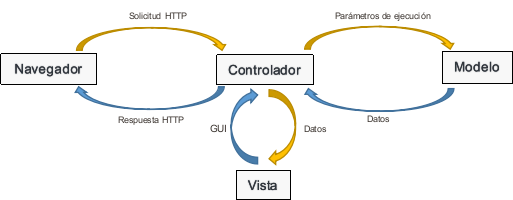
\includegraphics[width=0.7\linewidth]{Imagenes/MVC}
\end{figure}


Su funcionamiento es el siguiente, primero el usuario realiza alguna acción en la interfaz (por ejemplo, presiona un botón, un enlace, etc), luego el controlador recibe (por parte de los objetos de la interfaz-vista) la notificación de la acción solicitada por el usuario. El controlador gestiona el evento que llega, accediendo al modelo y actualizándolo, posiblemente modificándolo de forma adecuada a la acción solicitada por el usuario (por ejemplo, el controlador actualiza los datos del perfil del usuario) y después la interfaz de usuario espera nuevas interacciones del usuario, comenzando el ciclo nuevamente \cite{MVC2}.\\

Este patrón de diseño se usa en la programación orientada a objetos, por lo tanto se realiza la aplicación en el lenguaje de programación PHP, ya que es realmente útil para realizar la gestión de peticiones y envíos de formularios en dicha aplicación, además de que es importante también la gestión de las bases de datos de la aplicación, por este motivo se utiliza un framework basado en este lenguaje y esta arquitectura. Para gestionar las diferentes partes de la aplicación, en este caso se usa el framework Laravel, pues como se menciona anteriormente, está orientado a facilitar las tareas comunes de la mayoría de proyectos web que utilizan HTML5 y PHP.\\

Además, con este framework se hace uso de un ORM (Mapeo Objeto-Relacional) llamado Eloquent. Esta es una forma de mapear los datos que se encuentran en la base de datos a objetos de PHP y viceversa, esto facilita el uso de diferentes gestores de bases de datos como MySQL, SQLite, entre otras, ya que todas las consultas estan en PHP y el ORM ya se encarga del mapeo a los comandos SQL como se observa en la figura \ref{fig:orm}. Eloquent usa los modelos para enviar y recibir información de la base de datos\cite{Eloq}.\\

\begin{figure}[H]
	\centering
	\caption[ORM]{ORM [Imagen Propia]}
	\label{fig:orm}
	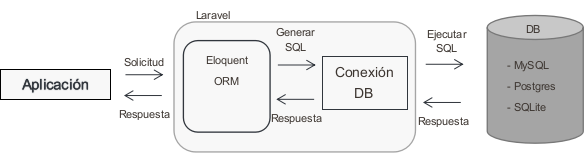
\includegraphics[width=0.7\linewidth]{Imagenes/ORM}
\end{figure}

\section{Prueba Beta}

Esta prueba se desarrolla en el entorno del cliente o usuario, arrojando resultados sobre las funcionalidades provistas para el software, además de dar la aceptación por parte del cliente si el producto funciona de manera adecuada o esperada \cite{PB}. Con el fin de realizar dicha verificación se analizan los objetivos a cumplir y los alcances, por lo tanto se separan los casos de prueba con el propósito de formular las preguntas que deben contestar las personas.\\

En general se ha propuesto el desarrollo de una solución IoT, con alcances como controlar cargas AC o DC y visualizar el estado del entorno de aplicación por medio de la pagina web desarrollada, por este motivo se presentan los diferentes casos de prueba a realizar y se menciona a continuación; las preguntas formuladas para estos se encuentran en el Anexo \ref{AnexoB}.

Prueba de conectividad de la tarjeta: La persona que participa en esta prueba debe realizar los primeros pasos para conectar la tarjeta con internet como se expone más adelante en resultados y se explica en Anexos en el manual de usuario.\\

De acuerdo con esto se califica la forma en que el cliente realiza este procedimiento, con la finalidad de analizar si es adecuada la manera en que se conecta la tarjeta SmartHouse a Internet por medio de Wi-Fi y también como reiniciar la conexión de la tarjeta para configurar nuevamente la red a la que se va a conectar. Las preguntas del número uno a la tres califican esta funcionalidad.\\

Prueba de la Aplicación Web: Evalúa el inicio de sesión, el monitoreo y control de todos los dispositivos que se encuentra conectados en tarjeta SmartHouse, además de las funcionalidades que posee el sistema en general.\\

Para esta prueba se deben realizar diferentes procedimientos, como iniciar sesión en la aplicación, encender o apagar un dispositivo, visualizar los datos de los sensores y configurar las reglas para los dispositivos. Las preguntas de la número cuatro en adelante califican estos aspectos y funcionalidades.\\

	\section{Resultados y Análisis}
\begin{frame}[t]
\frametitle{Resultados y Análisis}

En este capítulo se describen ciertos pasos y funcionamientos de la solución en general, para esto se supone una habitación con un sensor de temperatura, un ventilador y un bombillo led, las cuales el usuario va a visualizar y gestionar desde la aplicación web. En la figura \ref{fig:iot} está el esquema del sistema IoT.

\begin{figure}
	\centering
	\caption{Esquema Solución SmartHouse [Imagen Propia]}
	\label{fig:iot}
	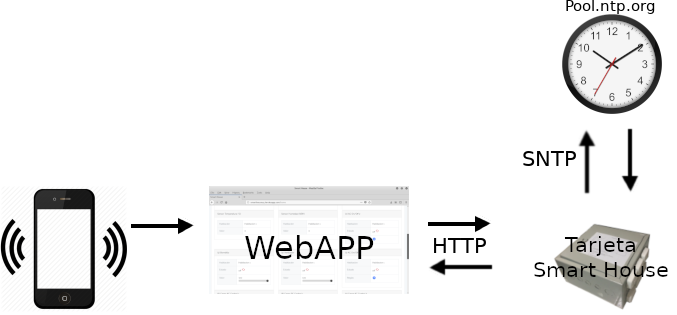
\includegraphics[width=0.6\linewidth]{Imagenes/IOT}
\end{figure}
\end{frame}

\subsection{Software}
\begin{frame}[t]
\frametitle{Resultados y Análisis}
\framesubtitle{Software}

Se desarrolla la aplicación web de manera local y posteriormente se lanza a un servidor en Internet. Se encuentra compuesta por los siguientes sitios y las diferentes interacciones basadas en las funciones básicas crear, leer, actualizar y borrar (CRUD).

\begin{itemize}
	\item Parte Pública
	\item Parte Privada
	\begin{itemize}
		\item Intercambio de datos
		\item Panel de Control
		\begin{itemize}
			\item Crear
			\item Ver
			\item Editar
			\item Eliminar 
		\end{itemize}
	\end{itemize}
\end{itemize}

\end{frame}

\begin{frame}[t]
\frametitle{Resultados y Análisis}
\framesubtitle{Software}
\footnotesize
De acuerdo con la lista anterior, se toman en cuenta dos partes, una pública y una privada, como se observa en la figura \ref{fig:index}. En la parte pública se encuentra una vista con la información de contacto del fabricante, solicitudes de registro o productos y la cantidad de usuarios que actualmente estan registrados en la aplicación. En la parte privada se encuentra la interacción de los usuarios sea administrador, dueño de una casa o de una habitación, para controlar y observar sus datos.

\begin{figure}
	\centering
	\caption{Página de Inicio. [Imagen Propia]}
	\label{fig:index}
	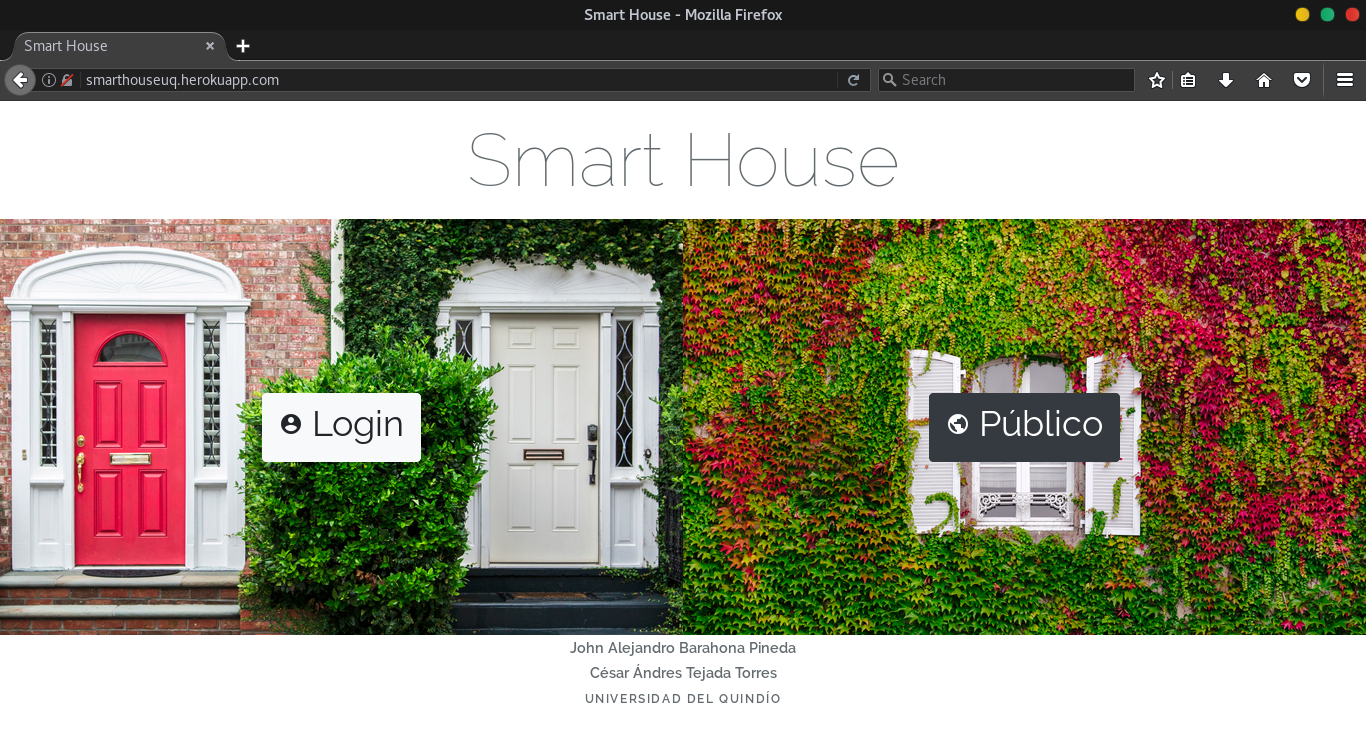
\includegraphics[width=0.6\linewidth]{Imagenes/Index}
\end{figure}

\end{frame}

\subsubsection{Parte Pública}

\begin{frame}[t]
\frametitle{Resultados y Análisis}
\framesubtitle{Software}

\textbf{Parte Pública: }
En esta vista únicamente hay opciones para el contacto y solicitudes, como se menciona anteriormente, es sencilla debido a la poca información que contiene, según se observa en la figura \ref{fig:publicview}.

\begin{figure}[H]
\centering
\caption{Vista Pública. [Imagen Propia]}
\label{fig:publicview}
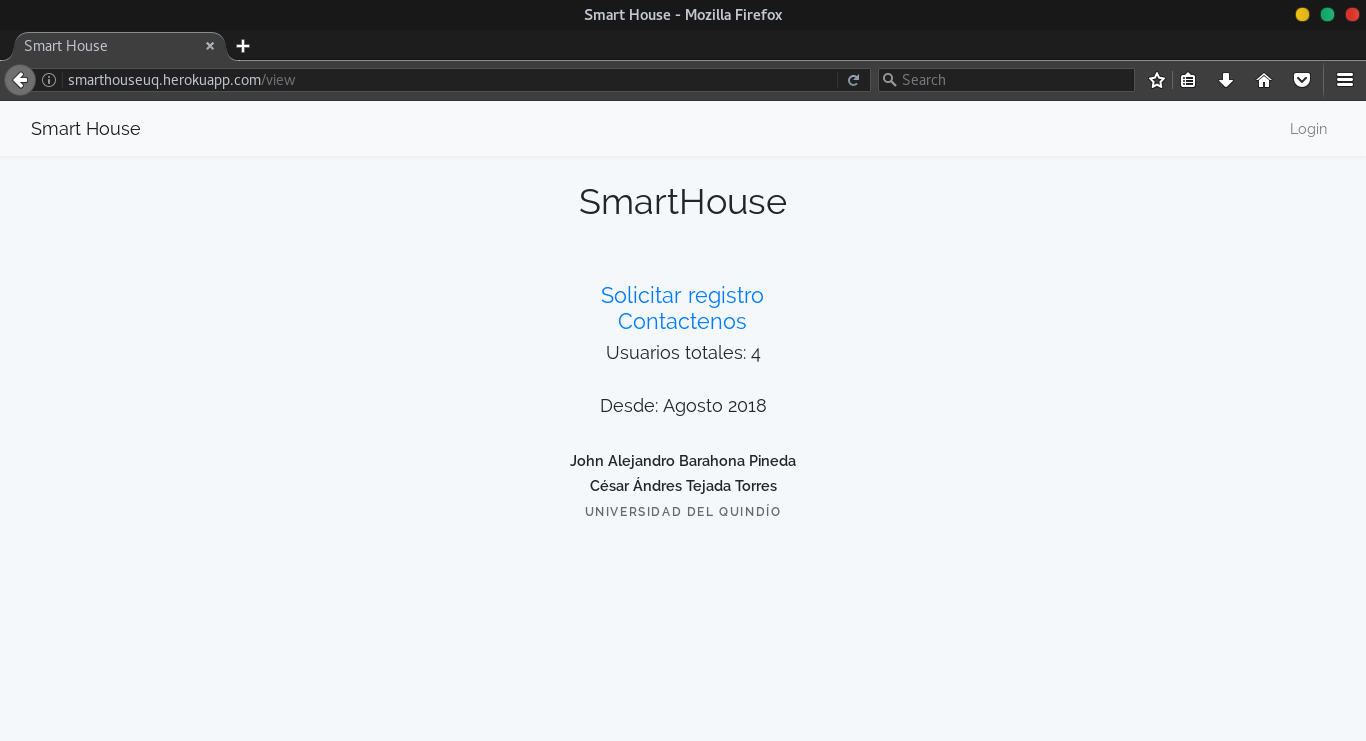
\includegraphics[width=0.5\linewidth]{Imagenes/Public_view}
\end{figure}

\end{frame}

\subsubsection{Parte Privada}

\begin{frame}[t]
En esta sección es donde se encuentra el Panel de Control para los diferentes usuarios de la aplicación. En primera instancia, un usuario administrador, el cual esta encargado de gestionar la aplicación, tiene la posibilidad de crear, ver, editar y eliminar los registros de la aplicación, la vista de este usuario se puede observar en la figura \ref{fig:views}\textbf{(a)}. Por medio de este se activan las cuentas de los demás, razón por la cual en la parte pública están las opciones de contacto y solicitud de registro.\\

También existe el usuario dueño de la vivienda donde se encuentra el dispositivo, este es opcional y es para gestionar los dispositivos presentes dentro de un mismo domicilio, es un administrador de la casa, el cual puede revisar y editar algunos campos de sus usuarios hijos o usuarios habitación y sus diferentes casas y habitaciones registradas a su nombre, como se ve en la figura \ref{fig:views}\textbf{(b)}, de este modo el rol de dicho usuario es administrar su hogar y visualizar los datos de esta.\\

Por último, otro rol es el de usuario habitación, el cuál únicamente visualiza sus propios datos, como la habitación y los dispositivos presentes en esta, según se observa en la figura \ref{fig:views}\textbf{(c)}, a este solo le compete la información de lo que posee en su cuarto, por tal motivo el panel de control muestra una vista general de los datos y el estado de sus dispositivos, además de tener la capacidad de editar partes básicas de su habitación y perfil. Dicho usuario puede o no estar sujeto a un usuario padre o usuario casa, ya que, solamente posee una tarjeta para su habitación y ninguna otra en dicha casa.\\

Continuando con este usuario y la habitación modelo propuesta al inicio del capitulo, luego de que accede a la aplicación web e inicia sesión con los datos que ha registrado en el sistema, al ser un usuario de una habitación, este se encuentra con un panel de control como el de la figura \ref{fig:views}\textbf{(c)}, allí gestiona los dispositivos presentes en su habitación, así como también puede visualizar la temperatura que se ha sensado y encender o apagar los dispositivos conectados a la tarjeta.\\

%\begin{figure}[H]
%	\centering
%	\caption{Vistas de Usuarios [Imagen Propia]}
%	\label{fig:views}
%	\subfigure[Usuario Administrador]{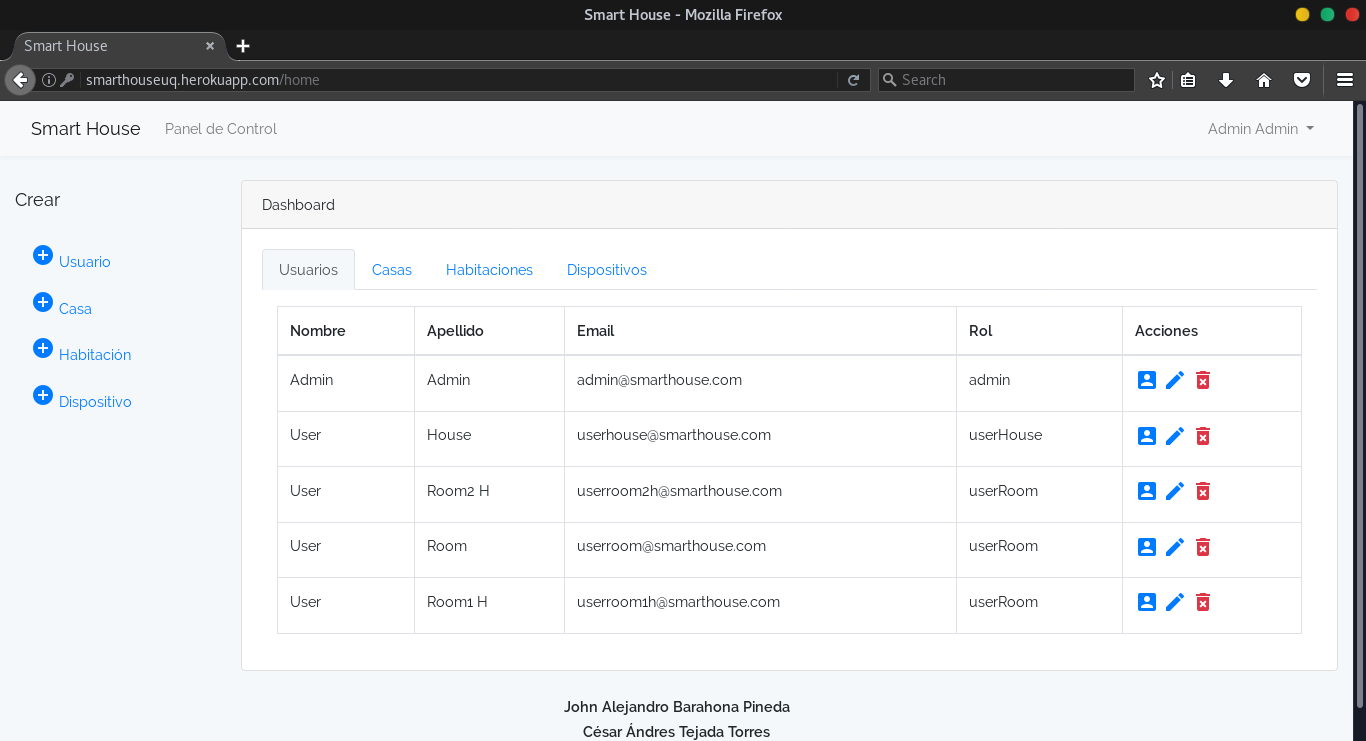
\includegraphics[width=0.9\linewidth]{Imagenes/Admin_view}}
%	\subfigure[Usuario de Casa]{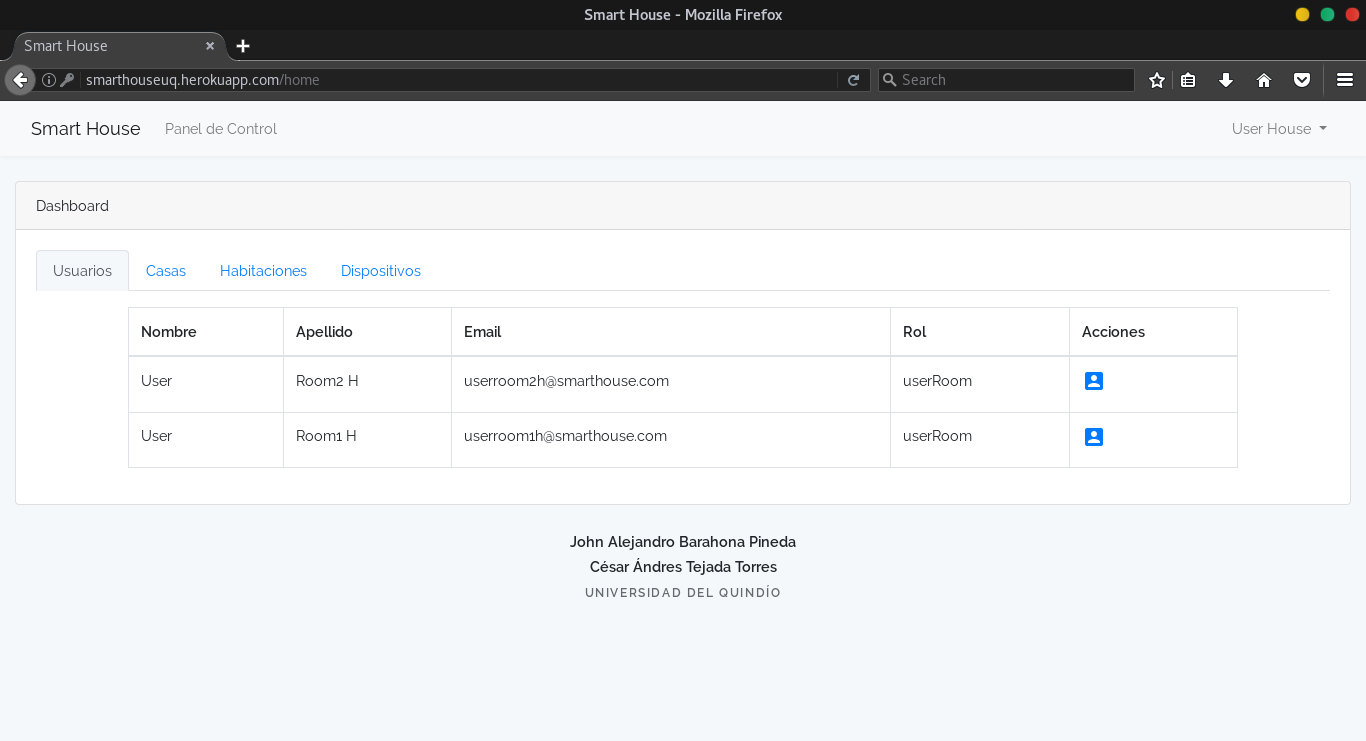
\includegraphics[width=0.45\linewidth]{Imagenes/UserH_view}}
%	\subfigure[Usuario de Habitación]{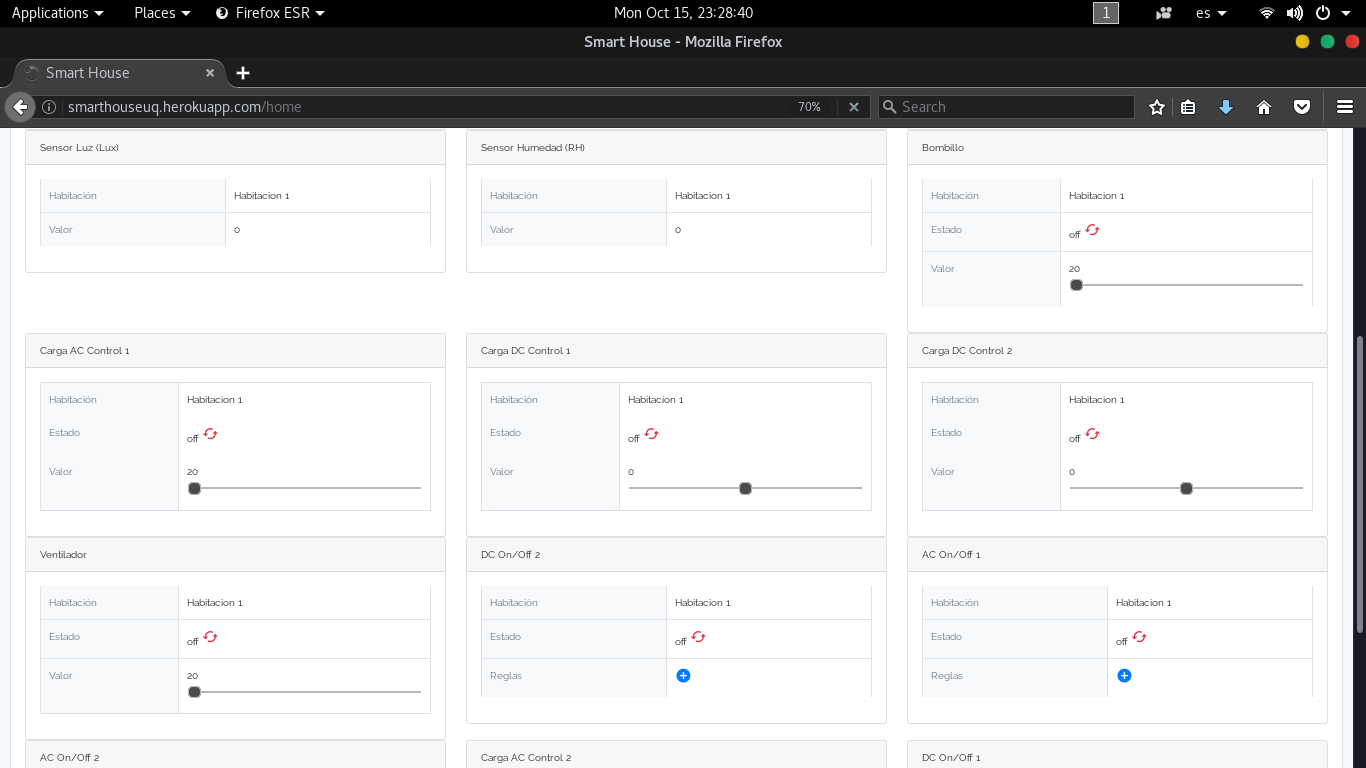
\includegraphics[width=0.45\linewidth]{Imagenes/UserR_view}}
%\end{figure}

\end{frame}

\begin{frame}

Además de este panel de control, desde el cuál se realizan las operaciones sobre la aplicación, en la parte privada se encuentra la ruta encargada de la actualización Servidor-Tarjeta, es decir, en esta ruta es donde se intercambia la información. Allí se realiza una petición HTTP tipo GET por parte de la tarjeta, incluyendo en su contenido el id de la habitación en la que está instalada, jutno con el token correspondiente a esta, además en la URL se añade un texto tipo JSON en el cual se ubican todas los datos de la lectura actual de los sensores; esta petición la responde el servidor con un texto también tipo JSON que contiene la información pertinente de las cargas o actuadores como se observa la figura \ref{fig:updateview}, para dar seguridad a dicha transacción, se se utiliza el token mencionado anteriormente, el cual se verifica mediante el id de la habitación comparando el recibido con el almacenado.\\

%\begin{figure}[H]
%	\centering
%	\caption{Página de intercambio de datos [Imagen Propia]}
%	\label{fig:updateview}
%	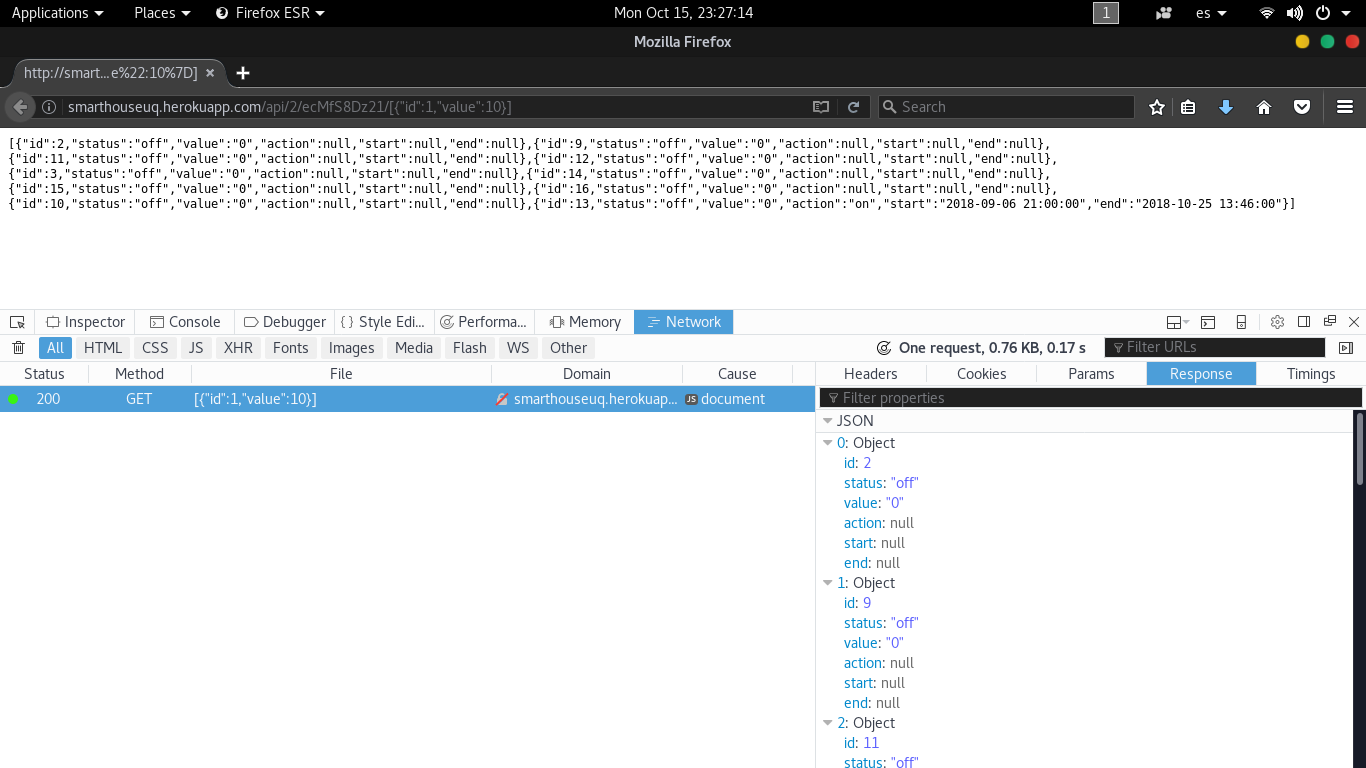
\includegraphics[width=0.7\linewidth]{Imagenes/Update_view}
%\end{figure}

\end{frame}

\begin{frame}
%De este modo, el usuario interactuando con la aplicación genera modificaciones en el texto con que responde el servidor a la petición de la tarjeta. Si el usuario desea encender el ventilador, como se observa en la figura \ref{fig:views}\textbf{(c)} esta presente un botón en la información del dispositivo, el cual con presionarlo lo enciende o apaga, esto es valido para cualquiera de los dos dispositivos, sea el ventilador o el bombillo led.\\
%
%Si el ventilador esta conectado a una salida de AC controlada, es posible que por medio del deslizador se le asigne un valor para que cambie su funcionamiento, del mismo modo ocurre con el bombillo led donde se refleja en su cambio de intensidad, pero este conectado a su respectiva salida DC controlada. Al generar estas interacciones el texto en formato JSON cambia de acuerdo con lo pedido por el usuario, modificando los campos de ``status'' y ``value'' en contraste con la acción realizada.\\ 

Adicional a esto, si el usuario desea añadir, modificar o eliminar una regla, por ejemplo, quiere encender el bombillo led a una hora deseada, esto lo puede lograr mediante el botón de reglas en el panel de control, el cual lo redirige a la vista que se observa en la figura \ref{fig:rulesview}, en esta se indica una hora de inicio y finalización en la que el bombillo led enciende a la hora de inicio y se apaga a la hora de fin, si es la regla de apagado solo necesita una hora de inicio para apagarlo.\\

%\begin{figure}[H]
%	\centering
%	\caption{Vista para añadir reglas [Imagen Propia]}
%	\label{fig:rulesview}
%	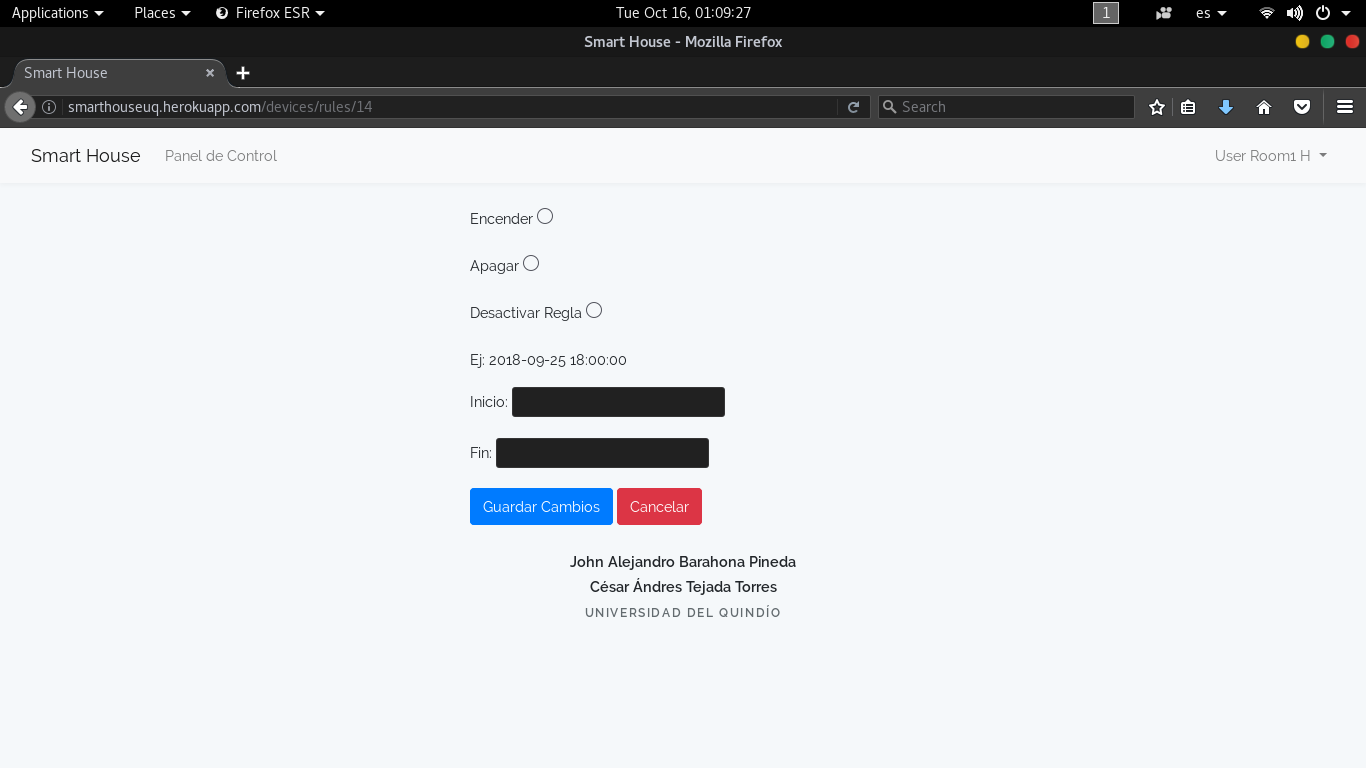
\includegraphics[width=0.6\linewidth]{Imagenes/rules_view}
%\end{figure}

\end{frame}

\begin{frame}
\subsubsection{Base de Datos}

La estructura de la base de datos se puede observar en la figura \ref{fig:db}, aquí se observan los diferentes campos que posee cada tabla, además de las llaves y sus relaciones. Las relaciones presentes en esta estructura son de tipo 1:N, es decir, por ejemplo un usuario puede tener relacionadas N casas.\\

%\begin{figure}[H]
%\centering
%\caption{Base de datos SmartHouse [Imagen Propia]}
%\label{fig:db}
%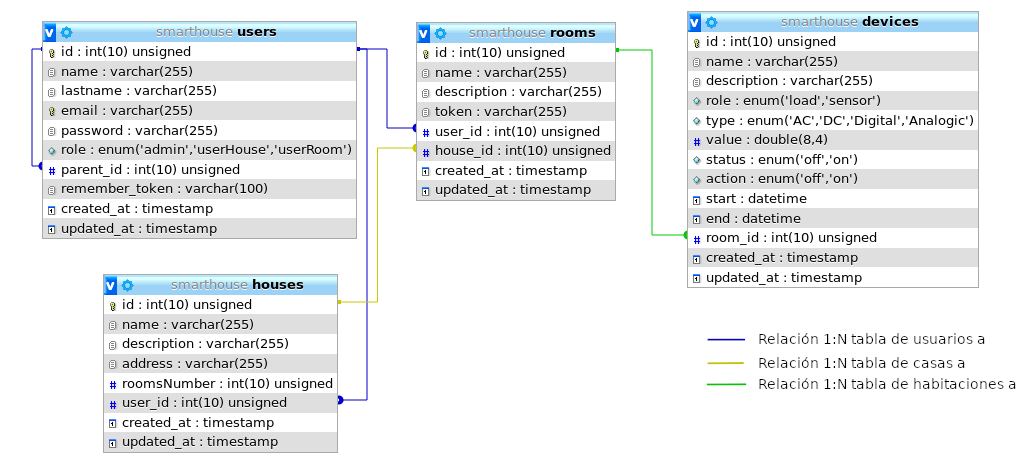
\includegraphics[width=0.75\linewidth]{Imagenes/DB}
%\end{figure}

%Esta sección donde se presentan todos los resultados en cuanto al software desarrollado presenta la mayoría de funciones implementadas en este, mostrando las diversas interfaces generadas en la aplicación, cumpliendo con los requisitos de permitir el monitoreo, control y la interacción del usuario con el dispositivo presente en su habitación, por medio de diferentes items que se han evidenciado en las figuras anteriores, permitiendo cambiar el estado de las salidas y asimismo visualizar los datos producidos por los sensores. También cabe resaltar que algunas salidas tienen la posibilidad de automatizarse a través de reglas, es decir, indicarle en que momento encender o apagar cierto dispositivo que se encuentre conectado a la tarjeta como se ha mencionado.\\

%Las funcionalidades para el cambio de estado en las salidas se realizan con cuidado, generando diálogos de confirmación con el fin de que el usuario este seguro de la acción que realiza. Para ejercer control sobre la energía entrega a las cargas, se cuenta con un deslizador o slider que permite cambiar el porcentaje de esta, asimismo es significativo resaltar que todos los datos generados de la interacción del cliente con el programa, se almacenan en la base de datos enlazada a dicha aplicación permitiendo una gestión adecuada de estos. Los resultados obtenidos del diseño de este software cumplen con el objetivo a partir del cual se construye y también se tienen algunas funciones adicionales como los usuarios administradores de casa, esto asegurando la escalabilidad de la aplicación. \\
%
%En cuanto a la protección de la aplicación se han mencionado los diferentes roles que se verifican por medio del middlware presente en esta solución, pero también cabe resaltar que con el objetivo de agregar seguridad a la transacción tarjeta-servidor se usa un token, el cual es único de cada habitación y se encuentra almacenado en la tarjeta y en el servidor, como se menciona anteriormente la aplicación al recibir la petición realiza esta verificación para proceder a contestar o simplemente ignorar la petición, de acuerdo con esto se esta ofreciendo un nivel de confiabilidad en dicha comunicación.\\

\end{frame}


\subsection{Firmware}
\begin{frame}

Como se ha mencionado anteriormente, el firmware se encuentra compuesto de tareas, en la figura \ref{fig:tareas} se observa un bosquejo del trabajo de las diferentes tareas, tomando por función principal la encargada de gestionar la conexión a Wi-Fi y almacenar sus credenciales, dependiendo del estado de si estan almacenadas o no, el sistema se comporta de una u otra forma. Si se encuentran credenciales guardadas en la tarjeta, el sistema se trata de conectar, si la conexión es exitosa comienza el proceso de actualización de la hora del sistema y también de las diferentes ordenes de la aplicación web. En cambio, si no existen credenciales el dispositivo inicia un servidor web local para que el usuario pueda proporcionarle esta información como se menciona en la sección \ref{sub:wifi}.\\

En cada caso se crean tareas diferentes, para el suceso de no existir credenciales únicamente se configura la tarea del servidor http local, y en la otra ocurrencia se lanzan todas la demás tareas encargadas de la escritura y lectura de datos, como se menciona en las siguientes secciones. Cabe resaltar que la tarjeta tiene disponible en promedio 160KB de memoria heap con el fin de poder realizar otras operaciones o implementar más funcionalidades en esta.\\

%\begin{figure}[H]
%	\centering
%	\caption{Esquema de Tareas [Imagen Propia]}
%	\label{fig:tareas}
%	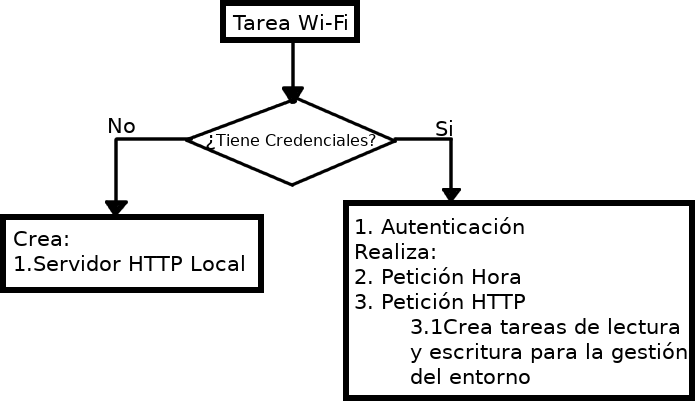
\includegraphics[width=0.7\linewidth]{Imagenes/tareas}
%\end{figure}
\end{frame}

\begin{frame}
Además de esto, se mide el promedio del tiempo en que se demora la ejecución de la tarea en dos casos, cuando realiza la primera petición después de conectado a la red, es decir, cuánto se tarda realizando las peticiones necesarias, como obtener la hora y fecha de la red y realizar la petición a la aplicación web, obteniendo una duración media de aproximadamente de 2.7s, esta depende de la disponibilidad de los diferentes servidores en la web asimismo de la velocidad y el tráfico de la red, ya que la tarjeta espera hasta que obtiene dicha hora y luego continua con la petición HTTP también esperando que el servidor responda. El otro caso es el lapso que se demora la tarea en leer los datos de los sensores, enviar la petición HTTP al servidor, recibirlos y enviarlos a los diversor actuadores, este periodo es de 1s en promedio, para conocer el dato se tomaron un total de 3056 muestras.
\end{frame}

\subsubsection{Conexión a Internet vía Wi-Fi}\label{sub:wifi}

Los sistemas IoT deben estar conectados siempre a Internet, por tal motivo se debe brindar una forma para conectar al sistema a este, en base a esto, se desarrolla un servidor local en la tarjeta que facilitar este proceso, como se ha mencionado el módulo del ESP32 funciona como Punto de Acceso (AP) y como Cliente o Estación (STA) al mismo tiempo, aprovechando esta capacidad se usa el servidor local y se encuentra encargado de gestionar la conexión de la tarjeta vía Wi-Fi como se observa en la figura \ref{fig:conexion}.\\

%\begin{figure}[H]
%	\centering
%	\caption{Conexión a Internet vía Wi-Fi ESP32 [Imagen Propia]}
%	\label{fig:conexion}
%	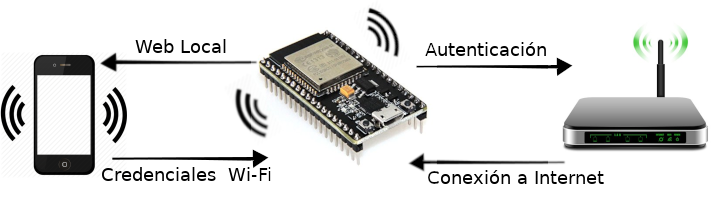
\includegraphics[width=0.7\linewidth]{Imagenes/conexion}
%\end{figure}


De este modo, en la figura \ref{fig:wifi} están algunas paginas del servidor local, en la figura \ref{fig:wifi}\textbf{(a)} es posible observar la lista de las diferentes redes al alcance de la tarjeta, basta con seleccionar una red e ingresar sus credenciales para conectarse, en la figura \ref{fig:wifi}\textbf{(b)} se observan los detalles de la conexión actual y también la opción de desconectarse. Su funcionamiento es muy intuitivo, se selecciona la red a la que se desea conectar la tarjeta, se ingresan sus credenciales y posteriormente el dispositivo verifica si la conexión fue exitosa o no; si lo es, la tarjeta esta lista para su funcionamiento, no obstante, se debe reiniciar para que solo quede funcionando como STA y no en el modo dual, además de esto si las credenciales de la red cambian, se incluye un botón para el borrado de estas, con el fin de que se puede configurar de nuevo el enlace con la red Wi-Fi.

%\begin{figure}[H]
%	\centering
%	\caption{Aplicación Conexión a Wi-Fi [Imagen Propia]}
%	\label{fig:wifi}
%	\subfigure[Lista de Redes]{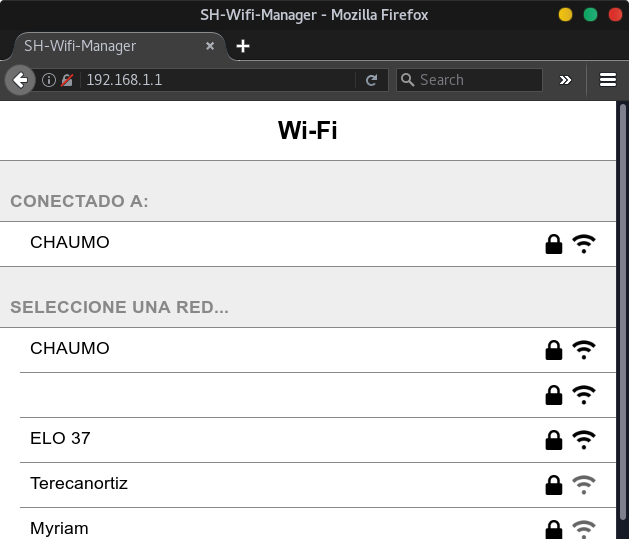
\includegraphics[width=0.45\linewidth]{Imagenes/w_status}
%		\label{fig:red}}
%	\subfigure[Datos de Conexión]{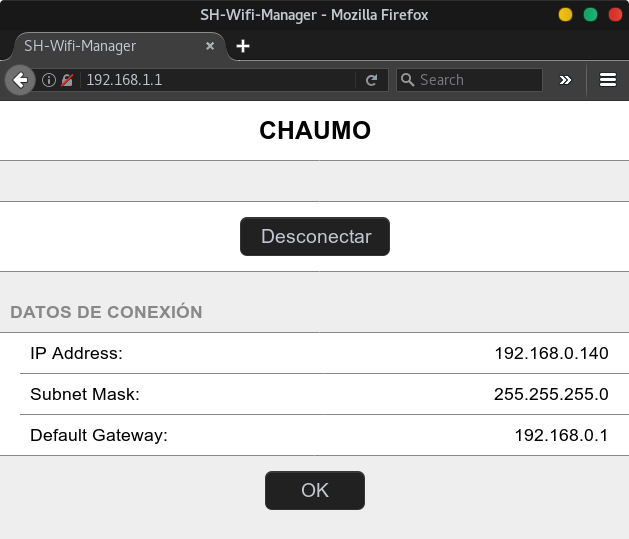
\includegraphics[width=0.45\linewidth]{Imagenes/w_red}
%		\label{fig:opt}}
%\end{figure}

\subsubsection{Escritura de Datos en la Aplicación Web}

Los datos que lee la tarjeta provienen de los diferentes sensores que tiene conectados según se ha mencionado, se usan diversos tipos, de estado para sensar la presencia, de calidad de aire entre otros presentes en esta. Para la escritura de los datos en el firmware se desarrollan varias tareas encargadas de leerlos y enviarlos a una tarea central. Los datos que están enviando contienen el id del dispositivo y la medida que lee en ese momento, estos se envían en forma de texto en formato JSON, de este modo, la tarea central los gestiona y envía a la aplicación con el mismo formato, organizandolos en la petición HTTP tipo GET que realiza, así la url que la tarjeta solicita, incluyendo el JSON de cada sensor, se observa en la figura \ref{fig:json}, de esta manera, en la url se encuentra el dominio del servidor, y la dirección que contiene el id y token de la habitación, por último se halla la información del sensor en formato JSON, que se compone por el id y el valor de este. La aplicación ya se encarga de almacenarlos y mostrarlos al usuario como se menciona anteriormente.

%\begin{figure}[H]
%	\centering
%	\caption{URL de la petición HTTP [Imagen Propia]}
%	\label{fig:json}
%	
\includegraphics[width=0.7\linewidth]{Imagenes/JSON}
%\end{figure}


\subsubsection{Lectura de Datos de Internet}

Para la configuración y comparación de las reglas que suministra el usuario a el dispositivo que desee controlar, es necesario contar con la hora actual y que se siga actualizando localmente gracias al RTC que posee internamente el ESP32, así, al inicio de la aplicación, se sincroniza y almacena la hora actual de la red, por medio del protocolo SNTP. Estas reglas actúan en cuanto a que encienda o apague un dispositivo en un instante dado, después de obtener este dato la ejecución programa continua con normalidad para realizar las diferentes peticiones a la aplicación web.\\

La interacción del usuario se da con la aplicación web mencionada anteriormente, de este modo la tarjeta siempre se debe actualizar, para esto, cuando la tarjeta envía los datos de los sensores, la aplicación responde con datos de cabecera HTTP y además la información de los dispositivos que controla la tarjeta, esta los recibe en una cadena texto en formato JSON como se observa en la figura \ref{fig:httprqstesp}, los procesa y los dirige a las tareas pertinentes ya sea para encender o apagar algún dispositivo conectado a la tarjeta, también remite las reglas que el usuario ha definido.\\

%\begin{figure}[H]
%	\centering
%	\caption{Respues del la APP Web a la Tarjeta [Imagen Propia]}
%	\label{fig:httprqstesp}
%	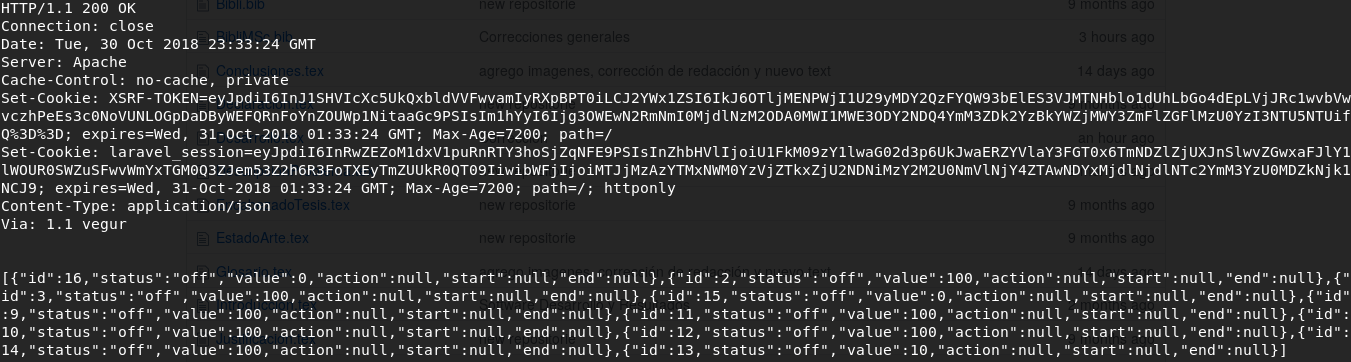
\includegraphics[width=0.8\linewidth]{Imagenes/HTTPRqstesp}
%\end{figure}

Según lo presentado en esta sección, la tarjeta cuenta con funcionalidades para conectarse con internet por medio de wi-fi, toda la configuración del cómo hacerlo la realiza el usuario mediante las herramientas ofrecidas por el programador, es decir, el servidor local. Durante el desarrollo de este programa se comprenden diferentes funciones que provee un RTOS, de manera que es viable haber desarrollado esta aplicación basado en este sistema operativo.\\

Analizando los tiempos de resolución de la petición http, siempre se tiene una media de 1s el cual es un tiempo de respuesta aceptable dadas todas las funcionalidades provistas en el programa, aunque este tiempo varia, ya que el haber utilizado el puerto serie para observar estos resultados, esta comunicación agrega también tiempo al procesamiento, así que es un aproximado, ya que asimismo interfiere la velocidad en la conexión a internet y la señal de recepción de wi-fi.\\

Por los resultados expuestos, el programa esta realizando correctamente las funciones necesarias para el monitoreo y control del ambiente de instalación, es decir, se cumple con los alcances provistos y además aún existen recursos de procesamiento para agregar nuevas funcionalidades o mejorar el desempeño.

\subsection{Hardware}

De acuerdo con los circuitos diseñados en la sección \ref{sec:hw} donde se propone el desarrollo de hardware de la solución IoT, en la figura \ref{fig:tarjeta} se observan las diferentes tarjetas ya ensambladas en una caja eléctrica para probar el funcionamiento del prototipo. Las salidas y entradas están distribuidas según lo propuesto, para las salidas AC se usan toma corrientes para conectar allí los diversos dispositivos, para las salidas DC se utilizan conectores hembra tipo banana para facilitar la conexión de estos dispositivos.\\

%\begin{figure}[H]
%	\centering
%	\caption{Tarjeta SmartHouse [Imagen Propia]}
%	\label{fig:tarjeta}
%	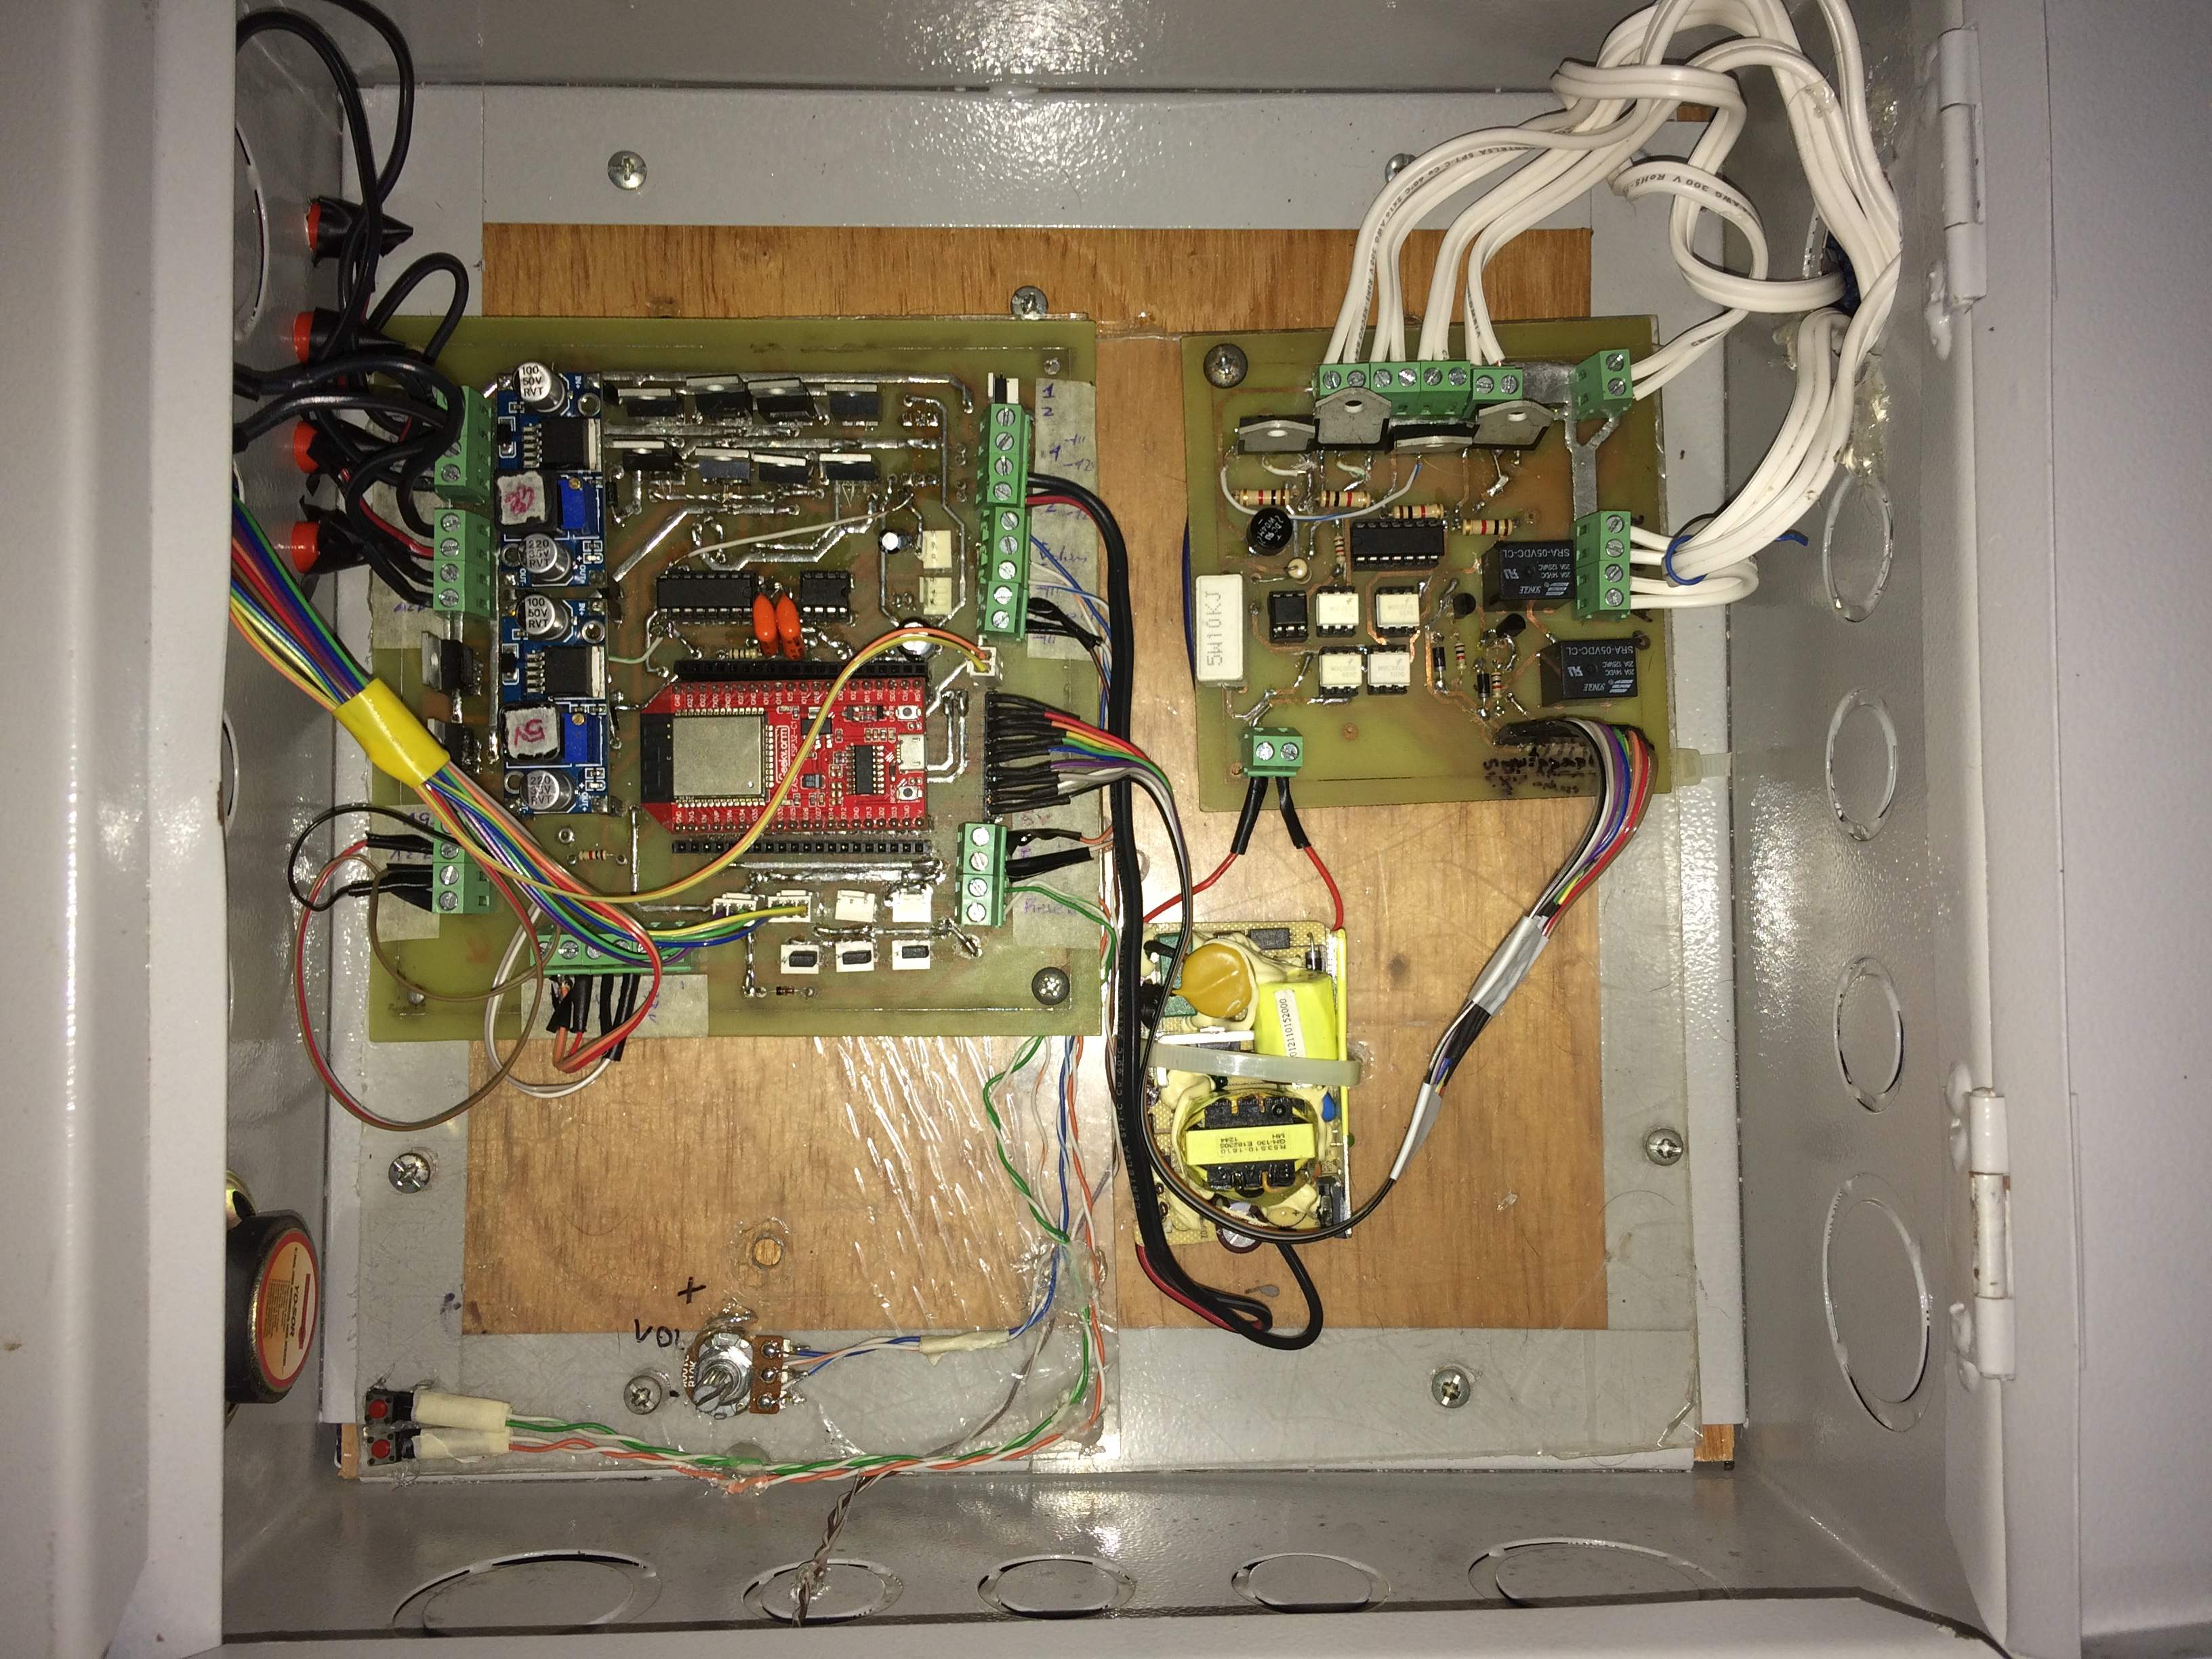
\includegraphics[width=0.6\linewidth]{Imagenes/Tarjeta}
%\end{figure}


La distribución de las diferentes salidas que posee la tarjeta se organizo en pegatinas y se colocaron sobre la caja eléctrica, la figura \ref{fig:labels} muestra esta información, tanto para la parte interna como externa de la caja.\\

%\begin{figure}
%	\centering
%	\caption{Descripción caja eléctrica tarjeta SmartHouse [Imagen Propia]}
%	\label{fig:labels}
%	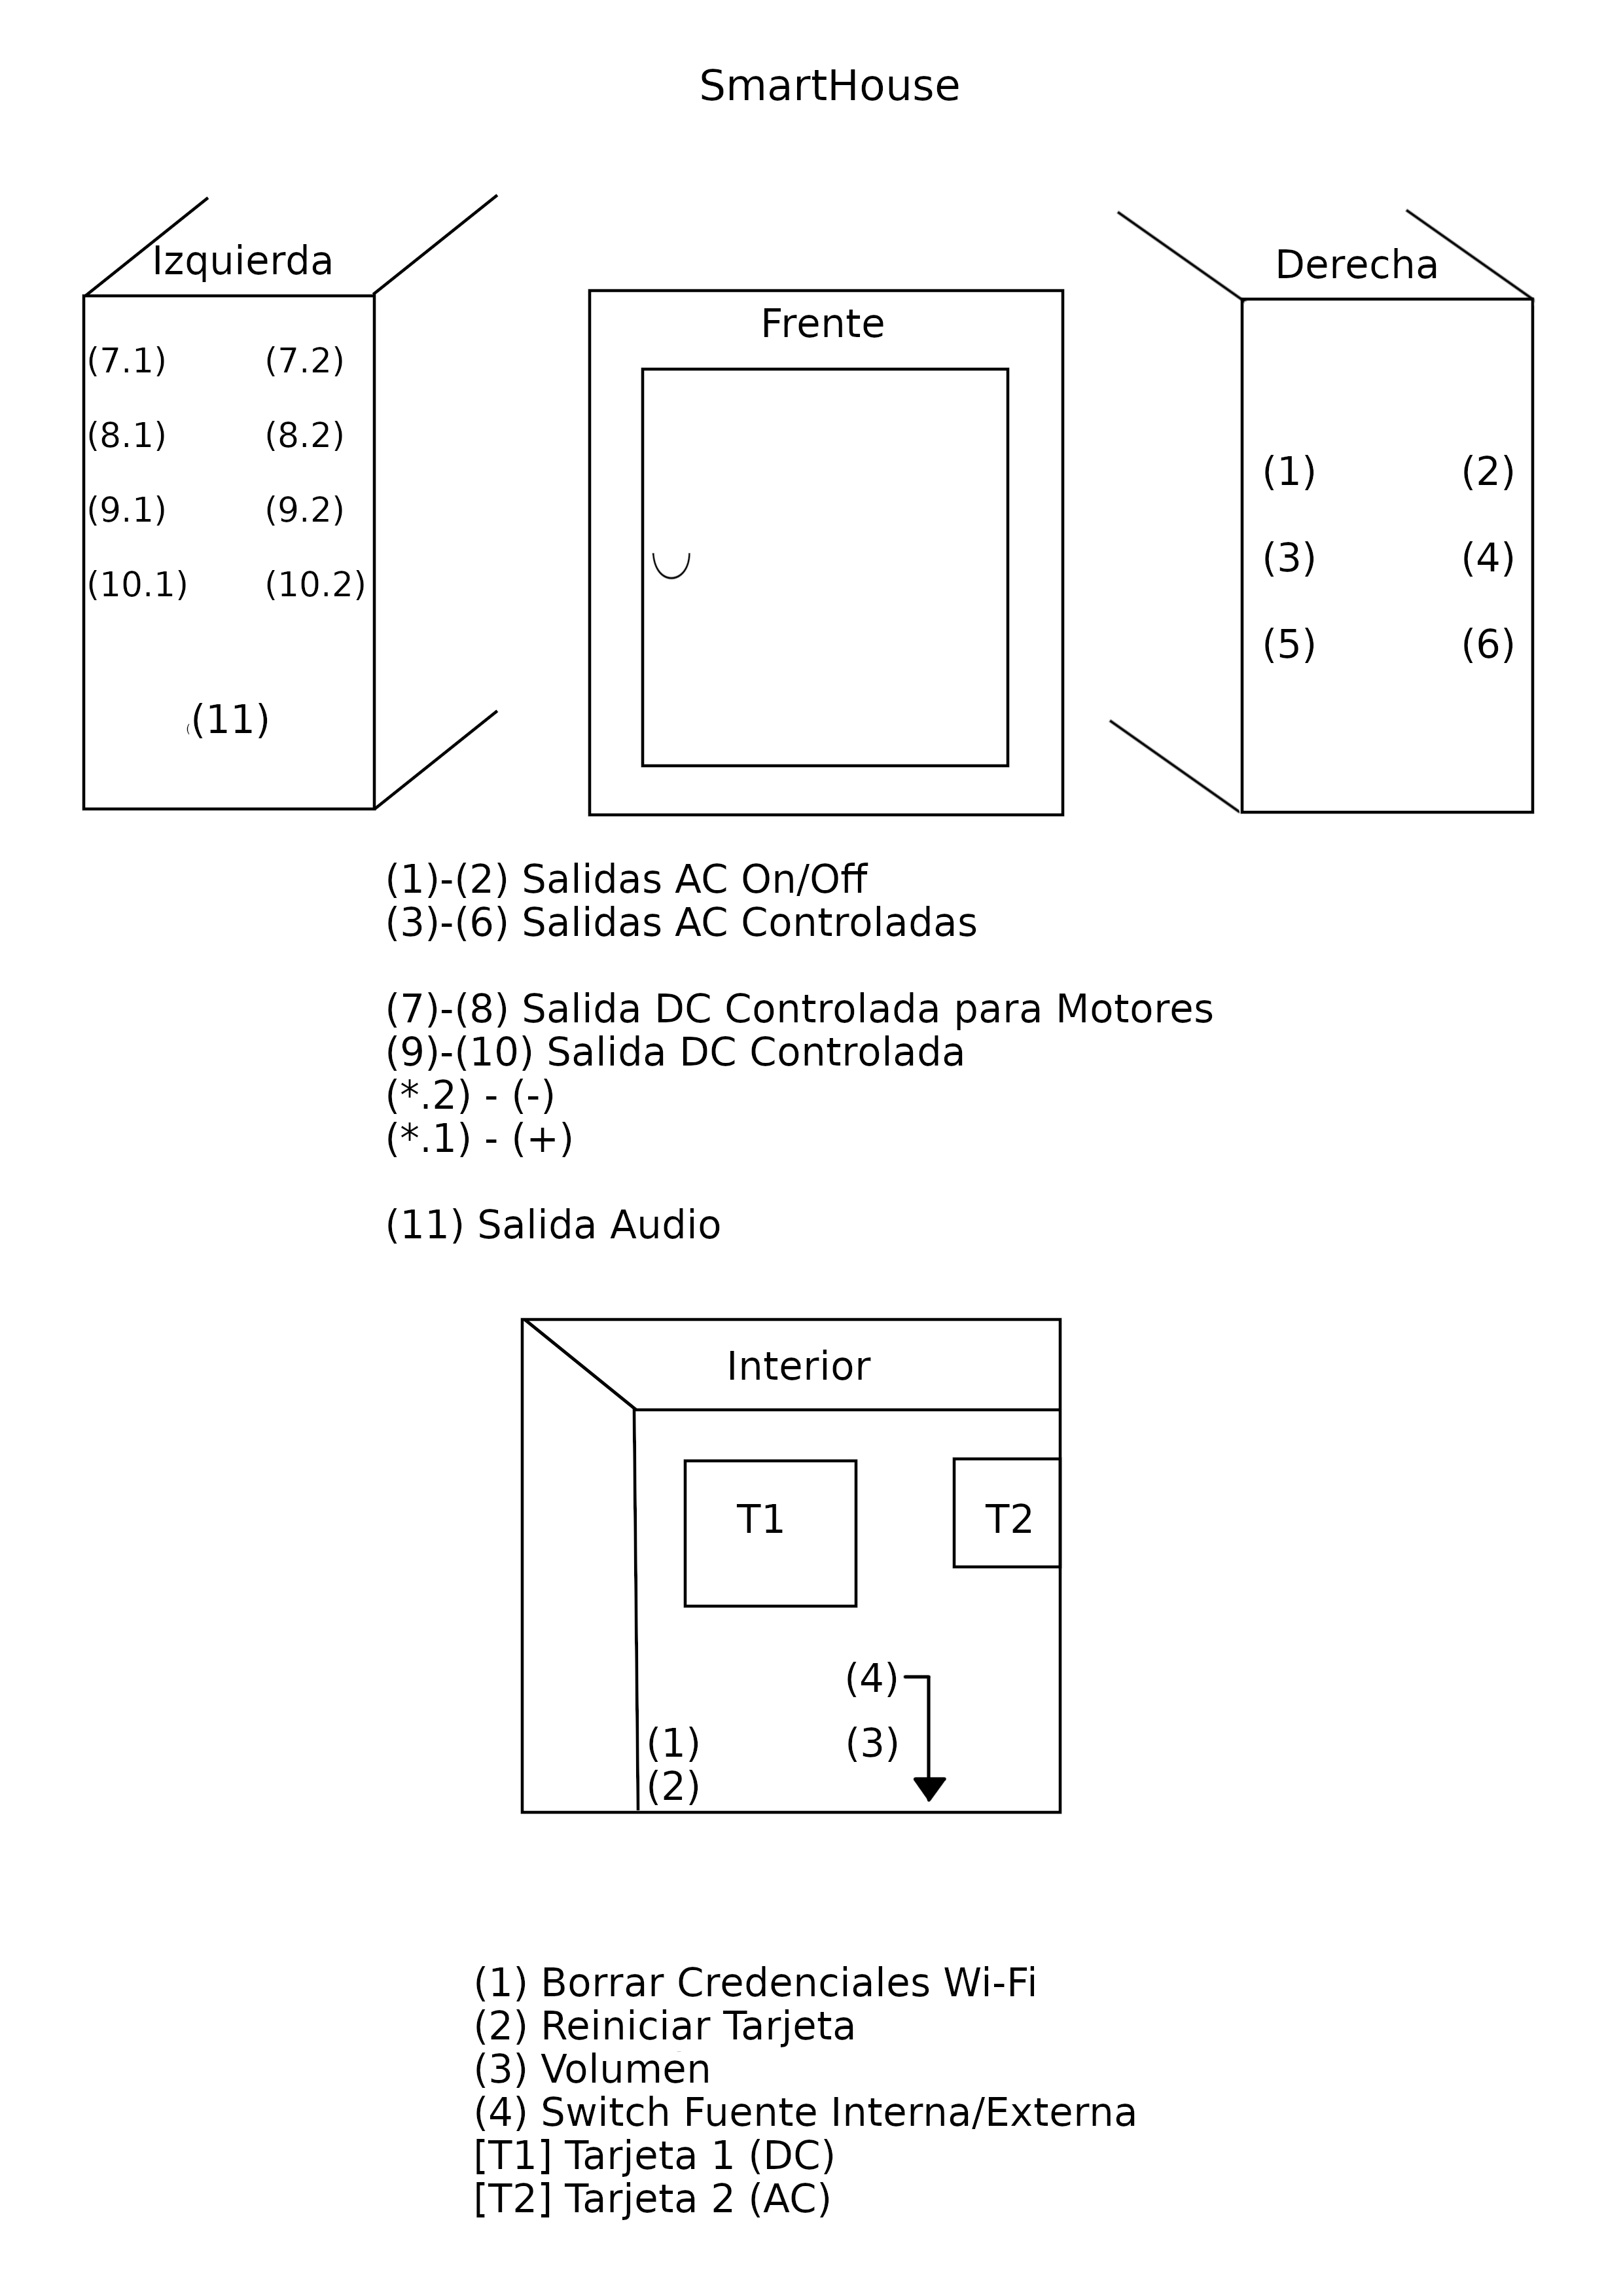
\includegraphics[width=0.7\linewidth]{Imagenes/labels}
%\end{figure}


Conforme a lo mencionado anteriormente, el sistema se ha probado con cargas AC como bombillos LED entre 7W y 20W, de filamento de 100W, probando funcionalidades como el control de potencia AC por ángulo de fase, obteniendo los resultados esperados, según se observa en la figura \ref{fig:ACc}\textbf{(a)} donde la carga tiene el 100\% de la potencia y en la figura \ref{fig:ACc}\textbf{(b)} con el 20\% de esta. El voltaje de alimentación viene dado por la red eléctrica, la tarjeta simplemente conmuta el estado de la alimentación o controla la potencia entregada. 

%\begin{figure}[H]
%	\centering
%	\caption{Control de potencia AC por ángulo de fase [Imagen Propia]}
%	\label{fig:ACc}
%	\subfigure[Potencia al 100\%]{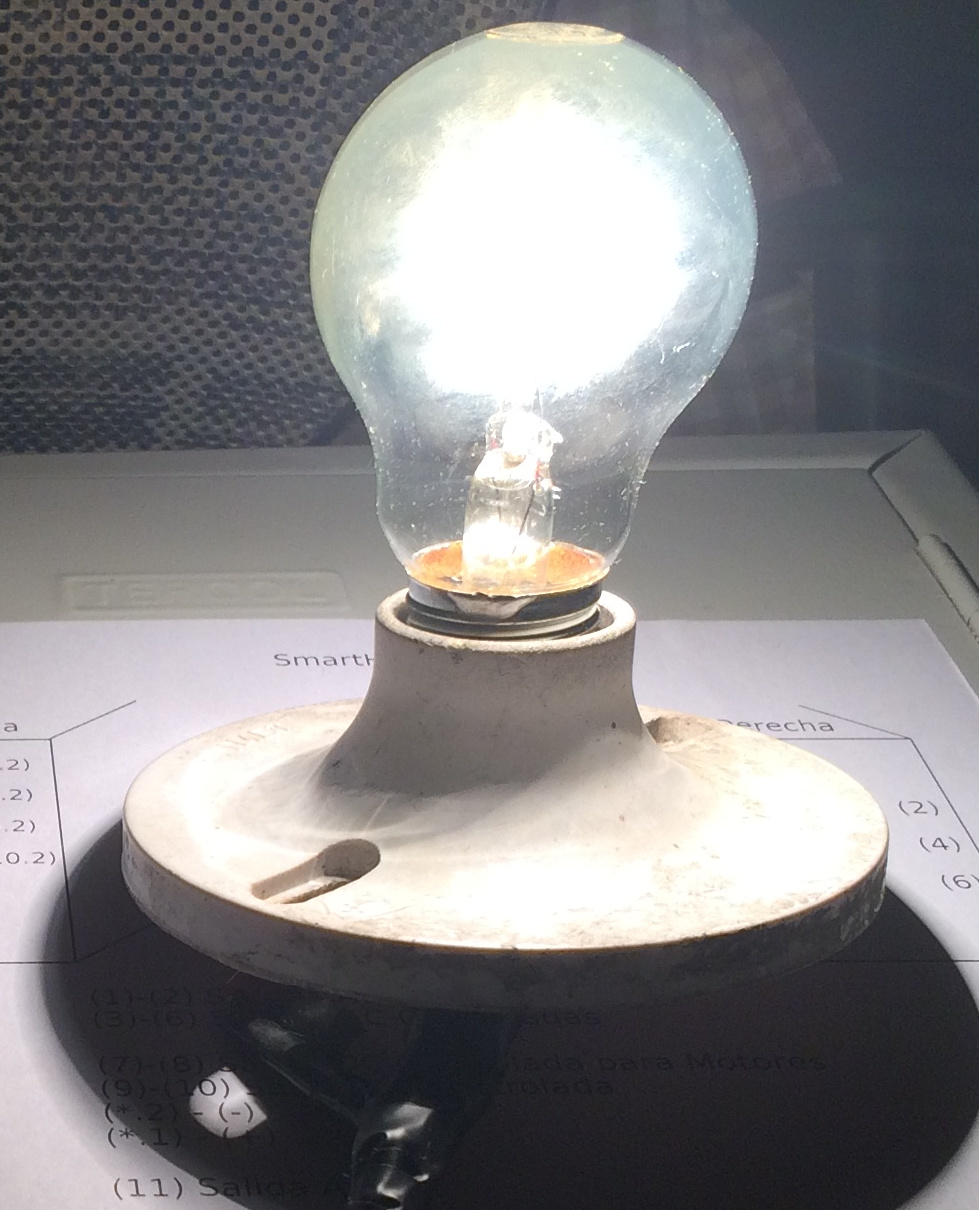
\includegraphics[width=0.45\linewidth]{Imagenes/AC1}}
%	\subfigure[Potencia al 20\%]{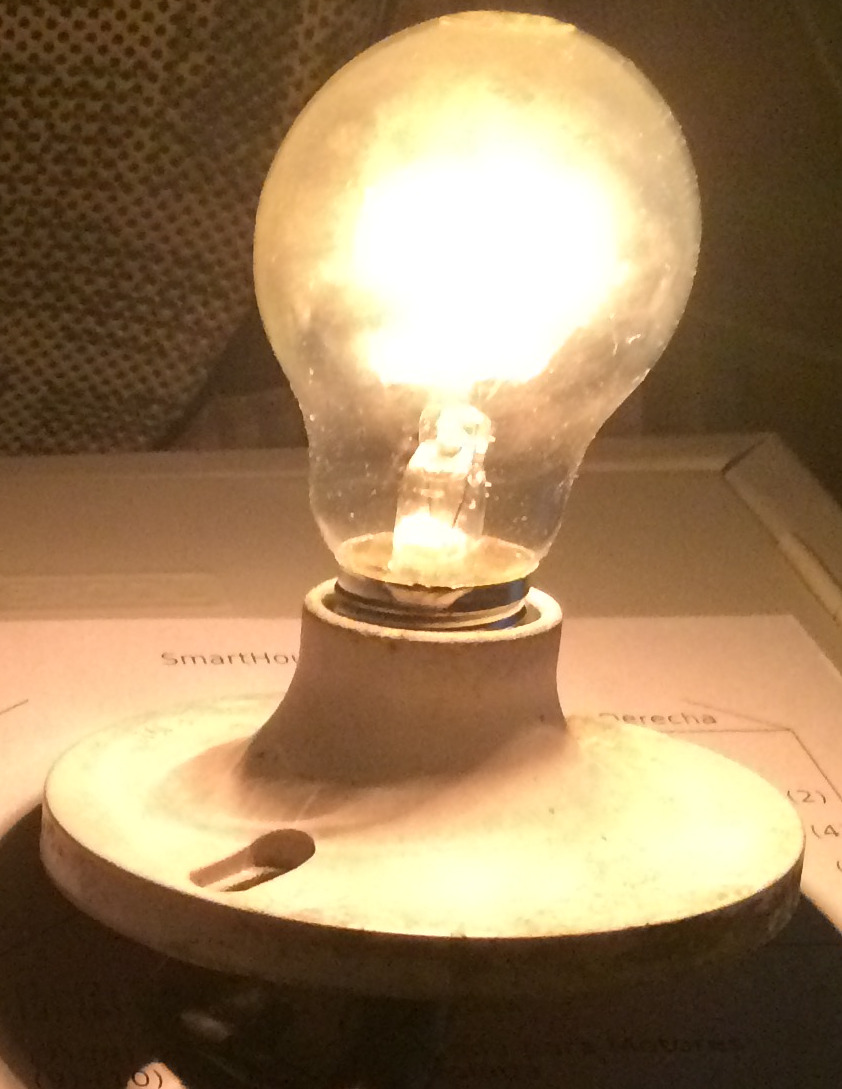
\includegraphics[width=0.43\linewidth]{Imagenes/AC0}}
%\end{figure}

Para las salidas DC se realizan pruebas con un motor DC de 1W, además de una tira LED de 1W, la cual se le varia la energía entrega, como se observa en la figura \ref{fig:DCc}\textbf{(a)} la carga tiene el 100\% de la energía y en la figura \ref{fig:DCc}\textbf{(b)} solamente el 10\%. Estas cargas se alimentan con 12VDC directamente desde la fuente o convertidor AC-DC, los circuitos que se implementan simplemente conmutan el estado de encendido/apagado o por medio de PWM variar la energía entregada.

%\begin{figure}[H]
%	\centering
%	\caption{Control de Cargas DC [Imagen Propia]}
%	\label{fig:DCc}
%	\subfigure[Potencia al 100\%]{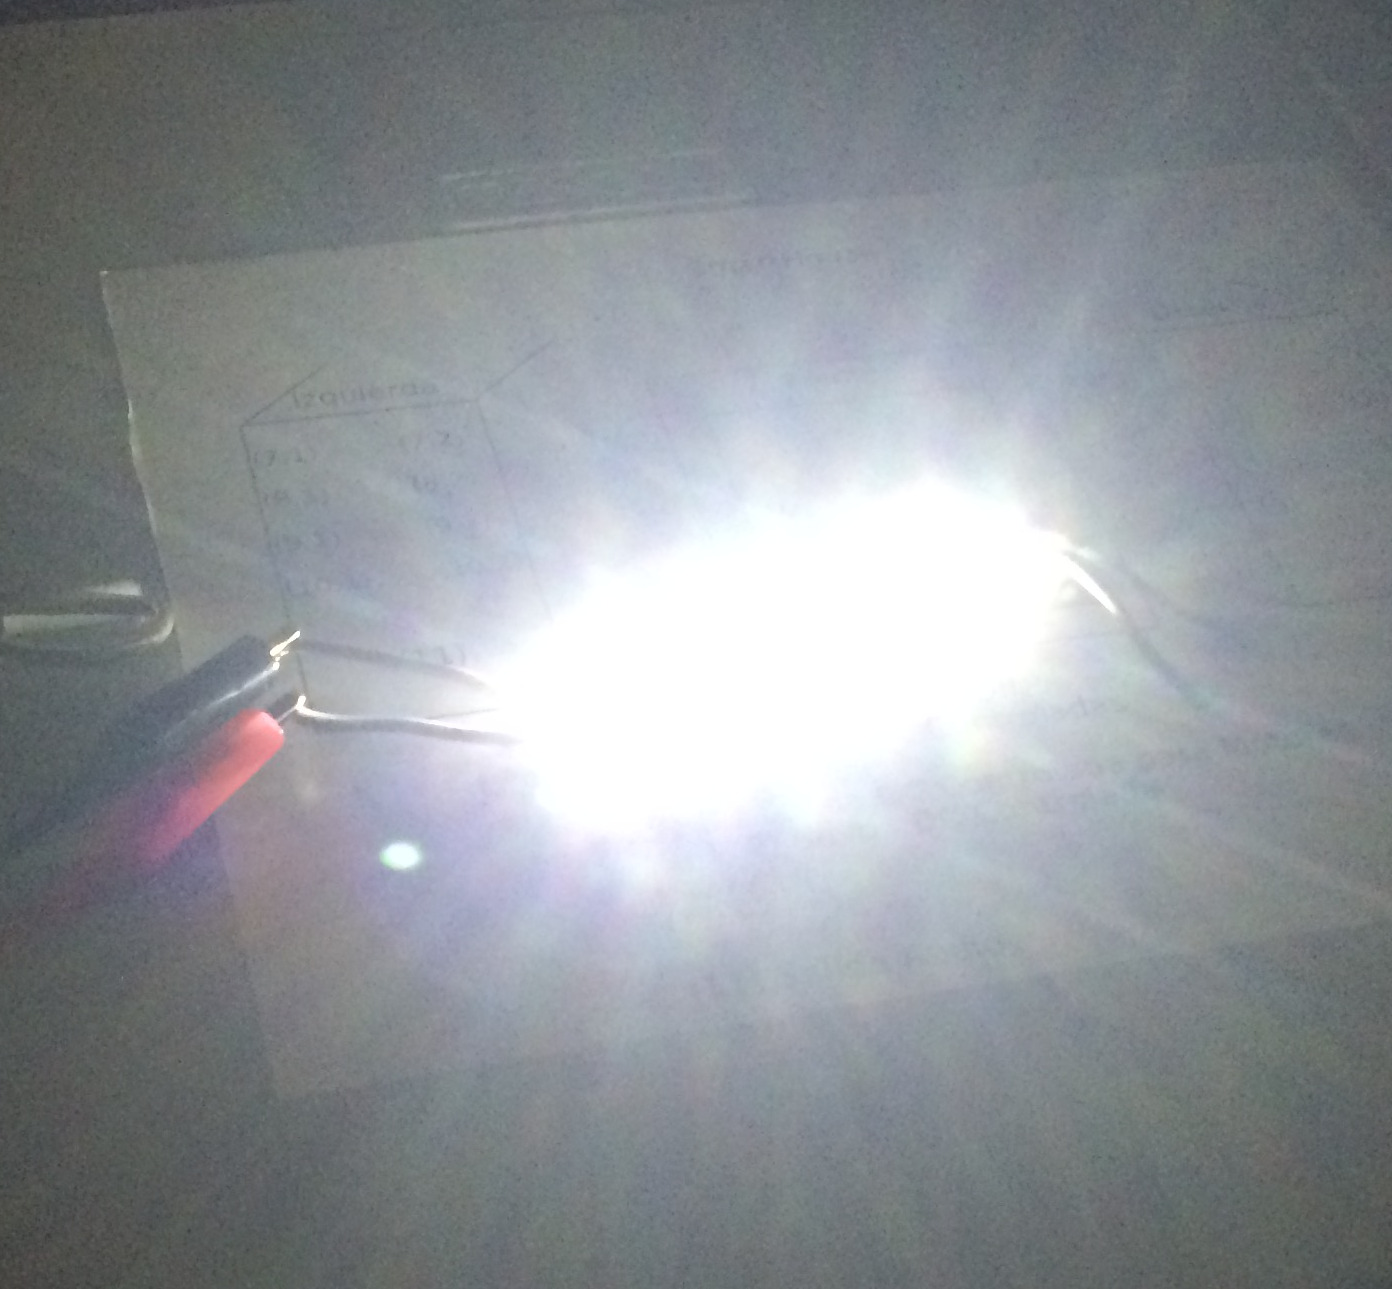
\includegraphics[width=0.45\linewidth]{Imagenes/DC1}}
%	\subfigure[Potencial al 10\%]{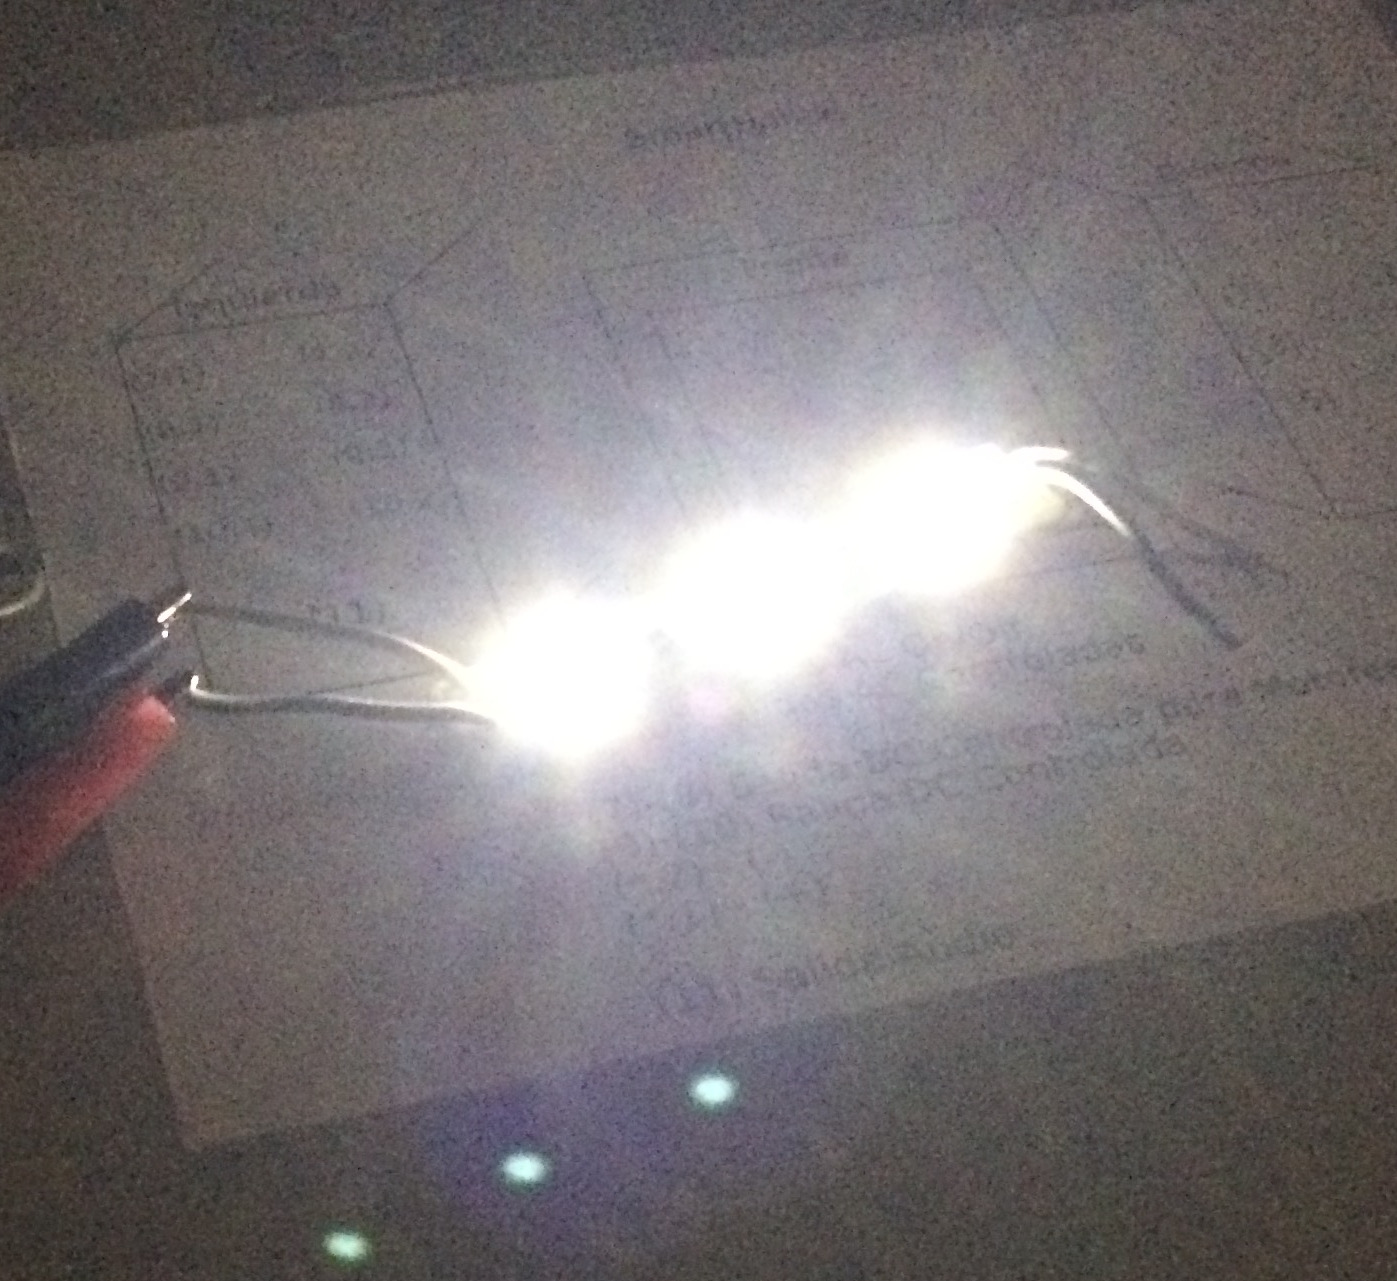
\includegraphics[width=0.455\linewidth]{Imagenes/DC0}}
%\end{figure}

En esta sección se evidencia tanto el hardware implementado, como su correcto funcionamiento de acuerdo con los requisitos propuestos, proporcionando las diferentes funcionalidades para que el firmware realice la gestión adecuada, es decir, controlar las salidas y recibir la información de los entradas. Se han construido diferentes circuitos, los cuales por medio del programa gestiona los diferentes dispositivos conectados a este.\\

Se observa que el hardware quedo dividido en dos tarjetas, esto para facilitar la construcción y distribución de los diferentes elementos utilizados, si se usan componentes superficiales y se aumentan las capas de la tarjeta es posible reducir el tamaño y hasta integrarlas en una sola board. En la construcción de estas tarjetas se comprende diferentes funcionamientos en cuanto a los triac y los transistores mosfet, reforzando conocimientos que se habían adquirido.\\

\subsection{Prueba Beta Cerrada}

Para la prueba beta se escoge un grupo de personas, las cuales interactuan directamente con la aplicación web y el prototipo de la tarjeta SmartHouse, se detallan los diferentes items a evaluar mencionados anteriormente, como el ingreso a la aplicación, visualización de los datos almacenados en esta y el control de los dispositivos.\\

Así, para evaluar estas características se formulan las siguientes preguntas, que se califican de acuerdo con una escala tipo likert \cite{lik} de uno a cinco en la cual, cinco es la calificación máxima y uno la mínima. Estas se formulan para evidenciar la postura del cliente en cuanto a las funcionalidades de la aplicación, conforme a esto la encuesta que se diseña esta presente en el Anexo \ref{AnexoB}, como se ha mencionado en la sección de desarrollo.\\

La prueba se realiza a quince personas, entre los cuales algunos son estudiantes de ingería electrónica y personas ajenas a este tipo de escenarios, los resultados de la prueba se consignan en la tabla \ref{table:enc} y también en el Anexo \ref{AnexoC} en forma digital, realizando el promedio de cada pregunta y presentando un resultado total, además en los anexos se encuentra el documento que cada persona respondió.\\

\begin{table}[H]
	\begin{center}
		\caption{Resultados por pregunta.}
		\label{table:enc}
		\begin{tabular}{|c|c|}
			\hline 
			\textbf{Número de la Pregunta} & \textbf{Promedio} \\ 
			\hline 
			1 & 4.5\\ 
			\hline 
			2 & 4.8\\ 
			\hline 
			3 & 4.5\\ 
			\hline 
			4 & 5.0\\ 
			\hline 
			5 & 4.9\\ 
			\hline 
			6 & 4.9\\ 
			\hline 
			7 & 4.3\\ 
			\hline 
			8 & 4.3\\ 
			\hline 
			9 & 4.8\\ 
			\hline 
			\textbf{Total} & \textbf{4.7}\\ 
			\hline 
		\end{tabular} 
	\end{center}
\end{table}

De acuerdo con los resultados es necesario analizar cada pregunta individualmente y también en su totalidad, así se pueden identificar las funciones a mejorar en el sistema. Con respecto al método de conexión de la tarjeta a Internet se obtiene un promedio de 4.5, indicando que los pasos que se deben cumplir para realizarlo están claros pero aún falta mejorar, esto sucede por la poca interacción que el usuario normalmente tiene con la configuración de dispositivos, de este modo se puede brindar ayuda telefónica o del servicio técnico en momento de la instalación.\\

Asimismo, la interfaz que se provee para realizar la conexión del sistema a la red Wi-Fi obtiene una calificación de 4.8, exponiendo que es de fácil uso pero faltan explicaciones en cuanto al momento de ingresar a esta, ya que se puede implementar también un DNS con la finalidad de que los usuarios no ingresen una dirección IP al navegador sino que escriban un nombre de dominio.\\

Además, em caso de que la red Wi-Fi cambie sus credenciales se provee un pulsador para eliminar estas, esta funcionalidad recibe una calificación de 4.5, algunos de los comentarios realizados sugieren el cambio de posición de este botón, ya que no se visualiza fácilmente y de una explicación un poco más detallada de esto, si es posible tener acompañamiento del personal técnico.\\

Después, al ingresar a la pagina web se presentan de manera clara los botones en la interfaz, es decir, el inicio de sesión obtiene una calificación de 5.0 lo que indica que para el usuario es fácil realizar dichas acciones, ya que los usuarios normalmente están muy familiarizados con estas, por ejemplo, cuando ingresan a redes sociales.\\

En cuanto a cómo se presenta la información de los diferentes dispositivos en el panel de control se obtiene 4.9, es decir, estos datos se presentan de manera clara y entendible para el usuario pero falta añadir un poco de explicación con el fin de que este se familiarice más con la interfaz propuesta.\\

Luego, en la parte de gestionar las salidas desde la web la calificación fue de 4.9, por lo tanto la manera en que se encienden, apagan y se controlan los diferentes dispositivos es claro, pero por ejemplo, por el tiempo de recarga automática de la página a veces es necesario cierta rapidez para cambiar alguna característica. Por tal motivo se modifica este lapso de 10s a 20s, de acuerdo con las observaciones realizadas.\\

Por otra parte, el tiempo de respuesta después de gestionar un dispositivo en la aplicación obtuvo 4.3, es una calificación baja respecto a las demás, este resultado depende de diversas circunstancias que se presenten durante la realización de la instrucción y todo lo que esto acarrea, desde el momento en que el usuario realiza la acción, es decir, que no coincida con la actualización automática de la pagina, la rapidez del navegador que posee el dispositivo desde el que realizan la actividad, entre otros factores también propios del programa, por ejemplo, el tiempo que la tarea esta suspendida o el lapso de ejecución de la instrucciones.\\

Respecto a la activación de las reglas para los dispositivos la calificación es de 4.3, ya que no es muy claro para el usuario qué es una regla dentro de la aplicación, además de que no están disponibles en todas las salidas por este motivo se puede mejorar la interfaz con el fin de definirlas de una mejor manera, asimismo hacerla más interactiva e intuitiva con el cliente.\\

Además, en una escenario general la facilidad de uso de la aplicación web recibe 4.8 como calificación, es decir que cumple con las expectativas, pero requiere agregar ciertos cambios para que sea más fácil de usar la primera vez que el cliente tiene contacto con esta. En este punto se resaltan observaciones ya mencionadas como el tiempo de actualización automática de la aplicación y la distribución del panel de control.\\ 

En resumen, la aplicación recibe una calificación de 4.7, por lo tanto se puede decir que las funcionalidades requeridas están programadas de una manera adecuada y simple para que el usuario disponga de ellas, pero es posible mejorarlas con el objetivo de que sean mucho más intuitivas para el usuario y que no se le presenten dudas al momento de usarla. Conforme a las observaciones obtenidas durante la prueba se han modificado algunas partes del sistema, que no tienen un impacto significativo sobre los objetivos ni alcances propuesto en este trabajo.\\

	\section{Conclusiones}

\begin{frame}[t]
\frametitle{Conclusiones}
\begin{itemize}
	\item El sistema compuesto de Firmware, Hardware y Software descrito en este documento es una solución IoT funcional, ya que este cuenta con la capacidad de monitorear y controlar un entorno de aplicación por medio de internet, el cual es en este caso una habitación de Smart House, siendo esta la representación de uno de los infinitos escenarios posibles a los cuales puede ser conectado el sistema, puesto que está diseñado con el fin de abarcar un amplio número de tareas, además de que acepta múltiples tipos de dispositivos de medida; combinando estos aspectos con una PaaS que permite la interacción humano-maquina, de tal manera que cumple con las características principales para una solución IoT.\\
\end{itemize}
\end{frame}


\begin{frame}[t]
\frametitle{Conclusiones}
\begin{itemize}
	\item El hardware implementado para la solución IoT, funciona en conjunto con el firmware que enlaza su parte física con el software presente en la nube; este fue diseñado en dos etapas con un circuito para cada una, las cuales son la etapa de potencia AC y la etapa DC. Esta organización del sistema no solo permite una clasificación en cuanto a su funcionamiento, sino que también evita que los altos voltajes de la etapa AC causen algún tipo de interferencia de manera directa con la etapa DC. Cada etapa del hardware cuenta con una alimentación que garantiza los niveles correctos para la alimentación de los sensores y cargas, además de una apropiada lectura de cada dispositivo de medida y una adecuada manipulación del entorno.\\
\end{itemize}
\end{frame}


\begin{frame}[t]
\frametitle{Conclusiones}
\begin{itemize}
	\item La aplicación web presentada en este documento, permite la interacción del usuario con los diferentes dispositivos que se encuentran conectados al hardware. Esta característica del sistema se encarga de la gestión de la información recolectada por el hardware junto con las órdenes administradas por el mismo, ya sea por visualización o manipulación del entorno de instalación, es decir, para su monitoreo o control, ya que se tiene acceso desde cualquier lugar con conexión a internet; de este modo la aplicación cumple con los diferentes alcances y puede seguir siendo ampliada a fin de adicionar funcionalidades al sistema. Con la implementación de este programa se han adquirido varios conocimientos sobre aplicaciones web y los lenguajes de programación que requieren, tales como PHP, JavaScript, entre otros.\\
\end{itemize}
\end{frame}


\begin{frame}[t]
\frametitle{Conclusiones}
\begin{itemize}
	\item La prueba Beta realizada para evaluar el sistema con la participación de los usuarios finales otorgo una calificación de 4.7, lo cual permite confirmar que se ha desarrollado de la mejor forma posible, desde el encendido y manipulación del hardware junto con sus conexiones, hasta la navegación a través de la aplicación web, facilitando estos procesos con ayuda de un manual de uso donde se encuentran indicados y detallados, ya que este fue escrito con la intención de ser entendido y seguido por cualquier usuario. Con esta puntuación se demuestra que aún quedan algunos pequeños aspectos por enriquecer, pero también indica que cumple con la funcionalidad propuesta, con el objetivo de mejorar se debe mantener un estrecho contacto con el cliente recibiendo constantes opiniones.\\
\end{itemize}
\end{frame}


\begin{frame}[t]
\frametitle{Conclusiones}
\begin{itemize}
	\item La tarjeta de prototipado ESP32 como unidad central de procesamiento dentro del desarrollo del hardware, representa una opción viable en la puesta en funcionamiento de un sistema IoT, no solo por su bajo costo sino también por sus características y funcionalidades, las cuales están diseñadas para este tipo de aplicaciones, permitiendo que el diseño y la implementación del sistema sea escalable, asimismo porque cuenta con un gran número de pines y diversas opciones para aumentar su capacidad.\\
\end{itemize}
\end{frame}


\begin{frame}[t]
\frametitle{Conclusiones}
\begin{itemize}
	\item El uso del framework ESP-IDF, que se compone de un sistema operativo en tiempo real freeRTOS, es muy útil para realizar las diferentes funciones del sistema que comunica hardware con software, además de que permite ejecutar las diversas tareas y gestionar bien los recursos presentes en el chip ESP32, por lo tanto es posible agregar una amplia gama de características adicionales a la funcionalidad del sistema, gracias a que esta en constante expansión agregando nuevas opciones y diversos controladores para el ESP32.\\
\end{itemize}
\end{frame}


\begin{frame}[t]
\frametitle{Conclusiones}
\begin{itemize}
	\item Se desarrolló una etapa de potencia AC que permite controlar las diferentes cargas presentes en una habitación, para esta se tiene un control de potencia por ángulo de fase el cual requiere de sincronización, precisión y un buen aislamiento del circuito con su unidad de control en este caso el ESP32. Por tal motivo se elige dicha tarjeta, ya que al poseer un RTOS es posible tener las características que brindan un correcto funcionamiento. Al implementar estos circuitos se han reforzado los diversos conocimientos obtenidos sobre los triacs y los distintos circuitos de aislamiento y activación para su uso.\\
	
\end{itemize}
\end{frame}

	\section{Trabajos Futuros}

\begin{frame}
\frametitle{Trabjos Futuros}

Como trabajo futuro en cuanto al hardware se propone integrar todo el sistema en una sola board, migrando la mayoría de componentes de montaje through hole a superficial (SMD) y también realizar un diseño con más capas, por ejemplo de cuatro capas, para reducir el tamaño de esta e incorporar todas las funcionalidades en una sola, además de añadir mas características a este, como el manejo de otros dispositivos por medio de infrarrojo, poder actualizar su firmware remotamente y funciones de ahorro de energía.\newline

En el software es conveniente agregar funcionalidades de acuerdo con los otros roles presentes en este, por ejemplo para el rol usuario administrador de casa crear reglas de control parental y de seguridad con el fin de ampliar la administración sobre sus propios dispositivos.\\

\end{frame}

\begin{frame}

En la parte de realización de la prueba del sistema se pueden realizar otros tipos como alfa, de aceptación, entre otras más que existen para probar los diferentes software diseñados, además ampliar la muestra en la que se aplican estas pruebas.\newline

Para mejorar la solución IoT es posible crear servidores espejo localmente en la tarjeta incluyéndolo en el firmware y realizando copias de la información constantemente. Sus funcionalidades son en caso de mantenimiento de la aplicación principal o de cualquier problema relativo a la conexión a Internet, esta daría soporte local hasta que entre de nuevo en funcionamiento la que se encuentra en la nube.\\
\end{frame}
 
\begin{frame}[allowframebreaks]
\frametitle{Bibliografía}
	\bibliographystyle{unsrt}
	\bibliography{BibliMSc}
\end{frame}
 
 %End Frame
 \setbeamertemplate{background canvas}{\includegraphics[width=\paperwidth,height=\paperheight]{Imagenes/final.jpg}}
 \begin{frame}

 \end{frame}


\end{document}
